\documentclass[12pt,a4paper,twoside]{article}
\usepackage[utf8]{inputenc}
\usepackage[acronym, toc, nonumberlist, nogroupskip]{glossaries}

\usepackage[english, polish]{babel}
\usepackage[OT4]{fontenc}
\usepackage{lmodern}
\usepackage{textcomp, gensymb}
\usepackage{float}

%%% fix for \lll
\let\babellll\lll
\let\lll\relax

\usepackage{amsmath}
\usepackage{mathtools}
\usepackage{amsfonts}
\usepackage{fancyhdr}
\usepackage{graphicx}
\usepackage{subfig}
\graphicspath{ {images/} }
\usepackage{amssymb}

\usepackage{enumitem}
\usepackage{scrextend}
\addtokomafont{labelinglabel}{\sffamily}
\usepackage{indentfirst}

\usepackage[hyphens]{url}
\usepackage[hidelinks]{hyperref}
\hypersetup{breaklinks=true}
\urlstyle{same}
%%% fix for \lll
\let\mathlll\lll
\let\lll\babellll

\usepackage[nottoc]{tocbibind}
\usepackage{bm}
\makenoidxglossaries
\usepackage{filecontents}
\glsnoexpandfields
\usepackage[numbers]{natbib}
\newcommand{\sectionbreak}{\cleardoublepage}

\setlength\headheight{15pt}
\enlargethispage*{0.7\baselineskip}




\pagestyle{fancy}
\fancyhf{}
\fancyfoot[LE,RO]{\thepage}

\fancyhead[LE]{Master's thesis - MICHALSKI Sz.}
\fancyhead[LO]{Star-tracker for small satellites}

\author{Szymon MICHALSKI}
\title{PROGRAM STAR-TRACKER DLA MAŁYCH SATELITÓW}


\begin{filecontents}{gloss.tex}
%================ACRONYMS=================%
\newacronym{adcs}{ADCS}{Attitude Determination and Control System}
\newacronym{ccd}{CCD}{Charge-Coupled Device}
\newacronym{cmos}{CMOS}{Complementary Metal–Oxide–Semiconductor}
\newacronym{dcm}{DCM}{Direction Cosine Matrix}
\newacronym{geo}{GEO}{Geostationary Orbit}
\newacronym{gnss}{GNSS}{Global Navigation Satellite System}
\newacronym{gps}{GPS}{Global Positioning System}
\newacronym{gso}{GSO}{Geosynchronous Orbit}
\newacronym{imu}{IMU}{Inertial Measurement Unit}
\newacronym{leo}{LEO}{Low Earth Orbit}
\newacronym{lis}{LIS}{Lost-In-Space}
\newacronym{meo}{MEO}{Medium Earth Orbit}
\newacronym{svd}{SVD}{Singular Value Decomposition}
%================SYMBOLS=================%
\newglossaryentry{phi}{type=symbols, name=$\phi$, sort=phi, description={Euler angle, roll}}
\newglossaryentry{theta}{type=symbols, name=$\theta$, sort=theta, description={Euler angle, pitch}}
\newglossaryentry{psi}{type=symbols, name=$\psi$, sort=psi, description={Euler angle, yaw}}
\newglossaryentry{euler_rotation_matrix}{type=symbols, name=$\bm{R}(\cdot)$, sort=euler_rotation_matrix, description={Rotation matrix using Euler angles}}
\newglossaryentry{unit_quaterion}{type=symbols, name=$\bm{q}$, sort=unit_quaterion, description={Unit quaternion}}
\newglossaryentry{scalar_quaternion_part}{type=symbols, name=$q_0$, sort=sigma, description={Scalar part of unit quaternion}}
\newglossaryentry{vector_quaternion_part}{type=symbols, name=$\bm{q}_{vec}$, sort=scalar_quaternion_part, description={Vector part of unit quaternion}}
\newglossaryentry{quaternion_matrix}{type=symbols, name=$\bm{Q}$, sort=quaternion_matrix, description={Quaternion matrix}}
\newglossaryentry{general_euler_angle}{type=symbols, name=$v$, sort=general_euler_angle, description={General Euler angle}}
\newglossaryentry{unit_vector}{type=symbols, name=$\bm{n}$, sort=unit_vector, description={Unit vector}}
\newglossaryentry{identity_matrix}{type=symbols, name=$\bm{I}$, sort=identity_matrix, description={Identity matrix}}
\newglossaryentry{skew_symmetrix_matrix}{type=symbols, name=$\bm{S}(\cdot)$, sort=skew_symmetrix_matrix, description={Skew symmetric matrix}}
\newglossaryentry{rotation_matrix}{type=symbols, name=$\bm{R}_n^b$, sort=rotation_matrix, description={Rotation matrix representing a rotation from n to b}}
\newglossaryentry{least_squares_estimate_rotation_matrix}{type=symbols, name=$\bm{M}$, sort=least_squares_estimate_rotation_matrix, description={Least squares estimate of rotation matrix}}
\newglossaryentry{unit_vector_ned}{type=symbols, name=$\bm{r}$, sort=unit_vector_ned, description={Known directional unit vector in the NED frame}}
\newglossaryentry{unit_vector_body}{type=symbols, name=$\bm{b}$, sort=unit_vector_body, description={Known directional unit vector in the BODY frame}}

\end{filecontents}

\newglossary{symbols}{sym}{sbl}{List of Symbols}
\makenoidxglossaries
\glsnoexpandfields
\loadglsentries{gloss.tex}


\begin{document}
\selectlanguage{english}

\begin{titlepage}
	\centering

	INSTITUTE OF CONTROL AND COMPUTATION ENGINEERING\par
	FACULTY OF ELECTRONICS AND INFORMATION TECHNOLOGY\par
	WARSAW UNIVERSITY OF TECHNOLOGY\par
	\vspace{0.5cm}
	
\includegraphics[scale=0.3]{logo_WEiTI.jpg}
	\hspace{1cm}
	
\includegraphics[scale=0.2]{Logo-PW-duze.jpg}
	\hspace{1cm}
	
\includegraphics[scale=1]{ia_600_600.png}
	\par
	\vspace{2cm}
	MASTER OF SCIENCE THESIS\par
	\vspace{0.2cm}
	{\huge STAR-TRACKER PROGRAM FOR SMALL SATELLITES\par}
	\vspace{0.2cm}
	{\large Szymon MICHALSKI\par}
	\vspace{3cm}
	\begin{flushright}
	Supervisor:\par
	prof. dr hab. inż. Ryszard Romaniuk\par
	\end{flushright}
	\vspace{6cm}
	{\large Warszawa 2019\par}
\end{titlepage}

\newpage
\thispagestyle{empty}
\phantom{a}
\vfill
\newpage
\thispagestyle{empty}

\begin{abstract}
Last years directed space industry towards small satellites. Many countries, which did not have possibility to enter this branch of industry before, now create their own solutions. The goal of this work is to create fully functioning star-tracker software eligible to be used in future satellites as Polish solution of determination of satellite attitude as well as research of possible usage of off-the-shelf embedded computer with GPU - NVIDIA Jetson TX2. Work contains also description of individual parts and variants of solutions connected with star-tracker.
\end{abstract}

\begin{otherlanguage}{polish}
\begin{abstract}
Ostatnie lata ukierunkowały przemysł kosmiczny na małe satelity. Wiele krajów, które wcześniej nie miały możliwości wejścia w tę gałąź przemysłu, teraz tworzy własne rozwiązania. Celem niniejszej pracy dyplomowej jest stworzenie w pełni działającego oprogramowania star-trackera nadającego się do wykorzystania w przyszłych satelitach jako polskie rozwiązanie problemu określania orientacji satelity, a także zbadanie możliwości użycia gotowego komputera wbudowanego z GPU - NVIDIA Jetson TX2. Praca zawiera też opis poszczególnych części i wariantów rozwiązania problemów związanych ze star-trackerem.
\end{abstract}
\end{otherlanguage}
\newpage
\thispagestyle{empty}
\phantom{a}
\vfill
\newpage
\pagenumbering{arabic}
\setcounter{page}{3}
\tableofcontents

\newpage
\setlength{\parindent}{1cm}
\setlength{\parskip}{\baselineskip}%



\glsaddall
\setlength{\glsdescwidth}{0.5\linewidth}
\setlength{\glspagelistwidth}{0.1\linewidth}

\printnoidxglossary[type=acronym,sort=letter]
\newpage

\printnoidxglossary[type=symbols,sort=use]

\newpage


\section{Introduction}
Stars were used for navigation already ages ago. Together with technological development, spread of sailing and seafaring people started to use more advanced tools helping to more precisely estimate position of ships on sea. In XVIII century new tool was created, named sextant. This device helped to quite precisely calculate angle between the line ship-horizon and ship-star, what let to estimate position.

Nowadays, hundreds of years later, thanks to other technologies like for example \gls{gps} stars are not necessary any more for traveling. As it is commonly known, \gls{gps} technology is based on satellites, and today those satellites need stars for determining their attitude towards Earth.

With the miniaturization of electronics and batteries new types of smaller satellites were invented: CubeSat and HyperSat. They have now greater sensory and processing power possibilities, previously found only in larger satellites, however they still need cheaper means of accurate attitude determination.

\subsection{Motivation}
The goal of this work is to make fully operational star-tracker software, that could be used on small satellites. Such program could be used on space missions and could start Polish state-of-the-art technology in growing space technology sector. The main focus is on the star identification part, as it is the most crucial part of the whole star-tracker, without which there would be no attitude determination possible.
Another part of the thesis is to research possibility of using off-the-shelf small computer NVIDIA Jetson TX2, as it would greatly lower the price of the hardware design and production, and it could be used together with software created during this work as complete star-tracker.

\newpage

\subsection{Outline of thesis}

This thesis consists of several chapters. Here they are shortly summarized:\par
\setlength{\parindent}{0cm}
\textbf{Chapter 1} serves as introduction to this thesis and describes the motivation and goal of this work. It also describes the background of the topic.\par
\textbf{Chapter 2} describes all the important foundations for the fully understanding given work.\par
\textbf{Chapter 3} describes how the star-tracker program works and goes through detailed comparison of different approaches.\par
\textbf{Chapter 4} describes the created prototype of star-tracker in Python language and performance on Jetson TX2\par
\textbf{Chapter 5} contains conclusions about this work and created star-tracker program, and about possible future work.\par
\textbf{Chapter 6} summarizes the work and describes possible future development of created star-tracker.\par

\setlength{\parindent}{1cm}

\subsection{Related work}

There exists a number of works connected to topic of star-tracker. Many works are cited later in this thesis as they describe important parts of algorithms. There are just a few works dealing with whole start-tracker program, not just parts of it, and nearly no works about whole program together with implementation on the real equipment. The related work can be divided into few sections:

\begin{itemize}[noitemsep]
\item Works describing small satellites in general: \citet{heidt2000cubesat} and \citet{swartwout2011brief}.

\item Algorithms for calculating star centroids: \citet{liebe2002accuracy}, \citet{samaan2002predictive}, \citet{knutson2012fast}, \citet{azizabadi2014vlsi}, \citet{lindh2014development} and \citet{zhang2014brightness}. 

\item Star identification (which star in image corresponds to which star in on-board catalogue) divided by design:
\begin{itemize}[noitemsep]
\item Grid Algorithm - \citet{padgett1997grid}, 
\item SP-Search - \citet{mortari1999sp},
\item Spherical Triangle - \citet{cole2004fast}, 
\item Pyramid - \citet{mortari2004pyramid}, 
\item Planar Triangle - \citet{cole2006fast}, 
\item Brightness Independent - \citet{dong2006brightness},
\item Geometric Voting - \citet{kolomenkin2008geometric}, 
\item Super k-ID and Multi Poles Algorithm created for ESA competition\cite{esa-competition},
\item use of neural networks: 
\begin{itemize}[noitemsep]
\item \citet{lindbladstar},
\item \citet{li2003star}, 
\item \citet{miri2012star}, 
\end{itemize}
\item separately discussed k-vector algorithm for faster search:
\begin{itemize}[noitemsep]
\item \citet{mortari1996fast}, 
\item \citet{mortari2000k},
\item \citet{mortari2013k}. 
\end{itemize}
\end{itemize}

\item Attitude Determination divided by design: 
\begin{itemize}[noitemsep]
\item Attitude estimation using Image Matching - \citet{delabie2012highly}, 
\item QUEST - \citet{shuster1990kalman}, 
\item Extended Quest - \citet{psiaki1999extended}, 
\item \gls{svd} - \citet{juang2003efficient},
\item EQUEST - \citet{rinnan2012development}, 
\item Optimal Image Matching - \citet{delabie2012highly}
\item QUEST improvement - \citet{cheng2014improvement}, 
\item summarized description of attitude estimation algorithms: 
\begin{itemize}[noitemsep]
\item \citet{markley1999estimate},
\item \citet{hall2003spacecraft},
\item \citet{tappe2009development}.
\end{itemize}
\end{itemize}

\item Works on hardware for star-tracker: \citet{felikson2011orbit}, \citet{azizabadi2014vlsi}, \citet{gaska2016obc}.

\item Works on full star tracker but without implementing on real device/ simulations only: \citet{rose2003star}, \citet{huffman2006designing}, \citet{diaz2006performance} and \citet{kandiyil2010attitude}.

\item Full star-tracker with device/on real device: \citet{mortari2002starnav}, \citet{cannata2007autonomous}, \citet{lizy2010str} and \citet{jalabert2011optimization}.

\end{itemize}

Many of those works will be mentioned and cited later in this thesis as they are crucial for this work and describe the ways how star-tracker should be designed. All those main algorithm types, like finding star centroids or star identification, are also described here in full detail in next sections.

It is also interesting to mention one work, which was done at Warsaw University of Technology together with Space Research Centre of Polish Academy of Sciences - Telegwiazda (eng. Telestar, rus. Telezvezda) - star-tracker designed for Gamma satellite, gamma ray telescope, in years 1978-90\cite{gamma-satellite}. That satellite was joint French-Soviet project with star-tracker made in Poland. Due to superior role of Soviet Union in that project comparing to Poland, the name of the star-tracker was changed to Russian (Telezvezda) and as such exists in international documents. Polish version of name exists only in Polish documents. There were two teams of scientists from Warsaw University of Technology working on this star-tracker: one from Faculty of Precision Mechanics under professor Romuald Jóźwicki designing optomechanical part of the system, and one from Faculty of Electronics under Grzegorz Czajkowski designing electronic part with on-board computer\cite{wut-space-research}.
The star-tracker was analyzing image of sky with FOV 9\degree . Four brightest stars in FOV were followed and their coordinates were sent to Earth, where they were compared with real star map. The software for checking stars' coordinates with real star map was created at Space Research Centre of Polish Academy of Sciences. star-tracker could register stars with magnitude equal or below 7 and with accuracy below 2 arcmin\cite{optical-devices-cbk}. Although the satellite failed shortly after its launch in 1990 due to power failure, star-tracker functioned properly and was among the few parts of the satellite which were functioning till the end of satellite's life in 1992. Comparing to Telegwiazda, modern star-trackers do not need to send stars' coordinates to Earth for comparing with sky map, but they can to this by themselves.


\subsection{Small satellites}

In recent years there has been the development of micro-satellites called CubeSats. CubeSat is a standard created in 1999 at the California Polytechnic State University\cite{heidt2000cubesat}, which is used for low-cost micro-satellites. CubeSats are measured in units. Most are 1U, 2U and 3U. CubeSat 1U has a size of 10 cm on each edge and the maximum weight of 1.333 kg, while the CubeSat 2U is 20x10x10 cm and can weigh up to 2.666 kg. CubeSat can have very low power supply for small units, but for units 6U and higher it can have from 17 Watts\cite{cubesat-panels} to even 126 Watts\cite{nanosat-tables}.

The advantage of the standard is primarily reduction of the price of elevation of such satellites into orbit. Their popularity is evidenced by the fact that the percentage of satellites weighing less than 10 kg has increased to about 60\% of all satellites, and only CubeSats make up about half of the small satellites that were launched in last years\cite{swartwout2011brief}\cite{swartwout2013first}. Till now there were around 1100 CubeSats launched\cite{nanosats}.

There exist wide range of CubeSat examples. Mostly they are scientific and students' satellites, for learning, experimental and science purposes. There are also few Polish examples: PW-SAT (1U) and PW-SAT 2 (2U) designed by students of Warsaw University of Technology, and Lem (8U) and Heweliusz (8U), both made at Polish Academy of Sciences. PW-SAT and PW-SAT 2 were used for learning and experimenting with new technologies, like deorbitation sail, solar sensor, etc.\cite{pw-sat2}.
Scientific satellites Lem and Heweliusz were built as part of BRITE programme - joint programme of Austria, Canada and Poland. The goal of this programme is to research mechanisms of energy transportation and angular momentum which happen inside hottest stars\cite{brite-pl}.

Typical CubeSat consist of many different components. Quite often it has antennas and radios for communication with mission centre on Earth, Electric Power System (subsystem responsible for managing electric power in the satellite), \gls{adcs} (subsystem responsible for analysing data from sensors and taking decision about trajectory, etc.), magnetometer, star-tracker, sun sensors, payload processor with mission instructions, etc. CubeSats are quite small, hence they usually do not have any propulsion system\cite{lemmer2017propulsion}. Figure \ref{fig:cubesat-build} shows the components of CubeSat on example of NASA's Interplanetary NanoSpacecraft Pathfinder In a Relevant Environment (INSPIRE).

\begin{figure}[!htbp]
  \centering
  \subfloat[PW-SAT\cite{pw-sat-image}]{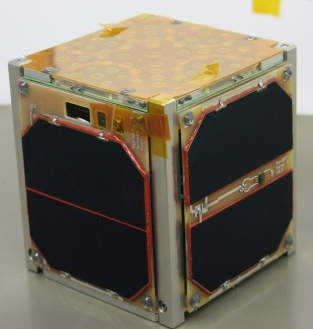
\includegraphics[width=0.4\textwidth]{pw-sat.jpg}\label{fig:pw-sat}}
  \hfill
  \subfloat[PW-SAT 2\cite{pw-sat2}]{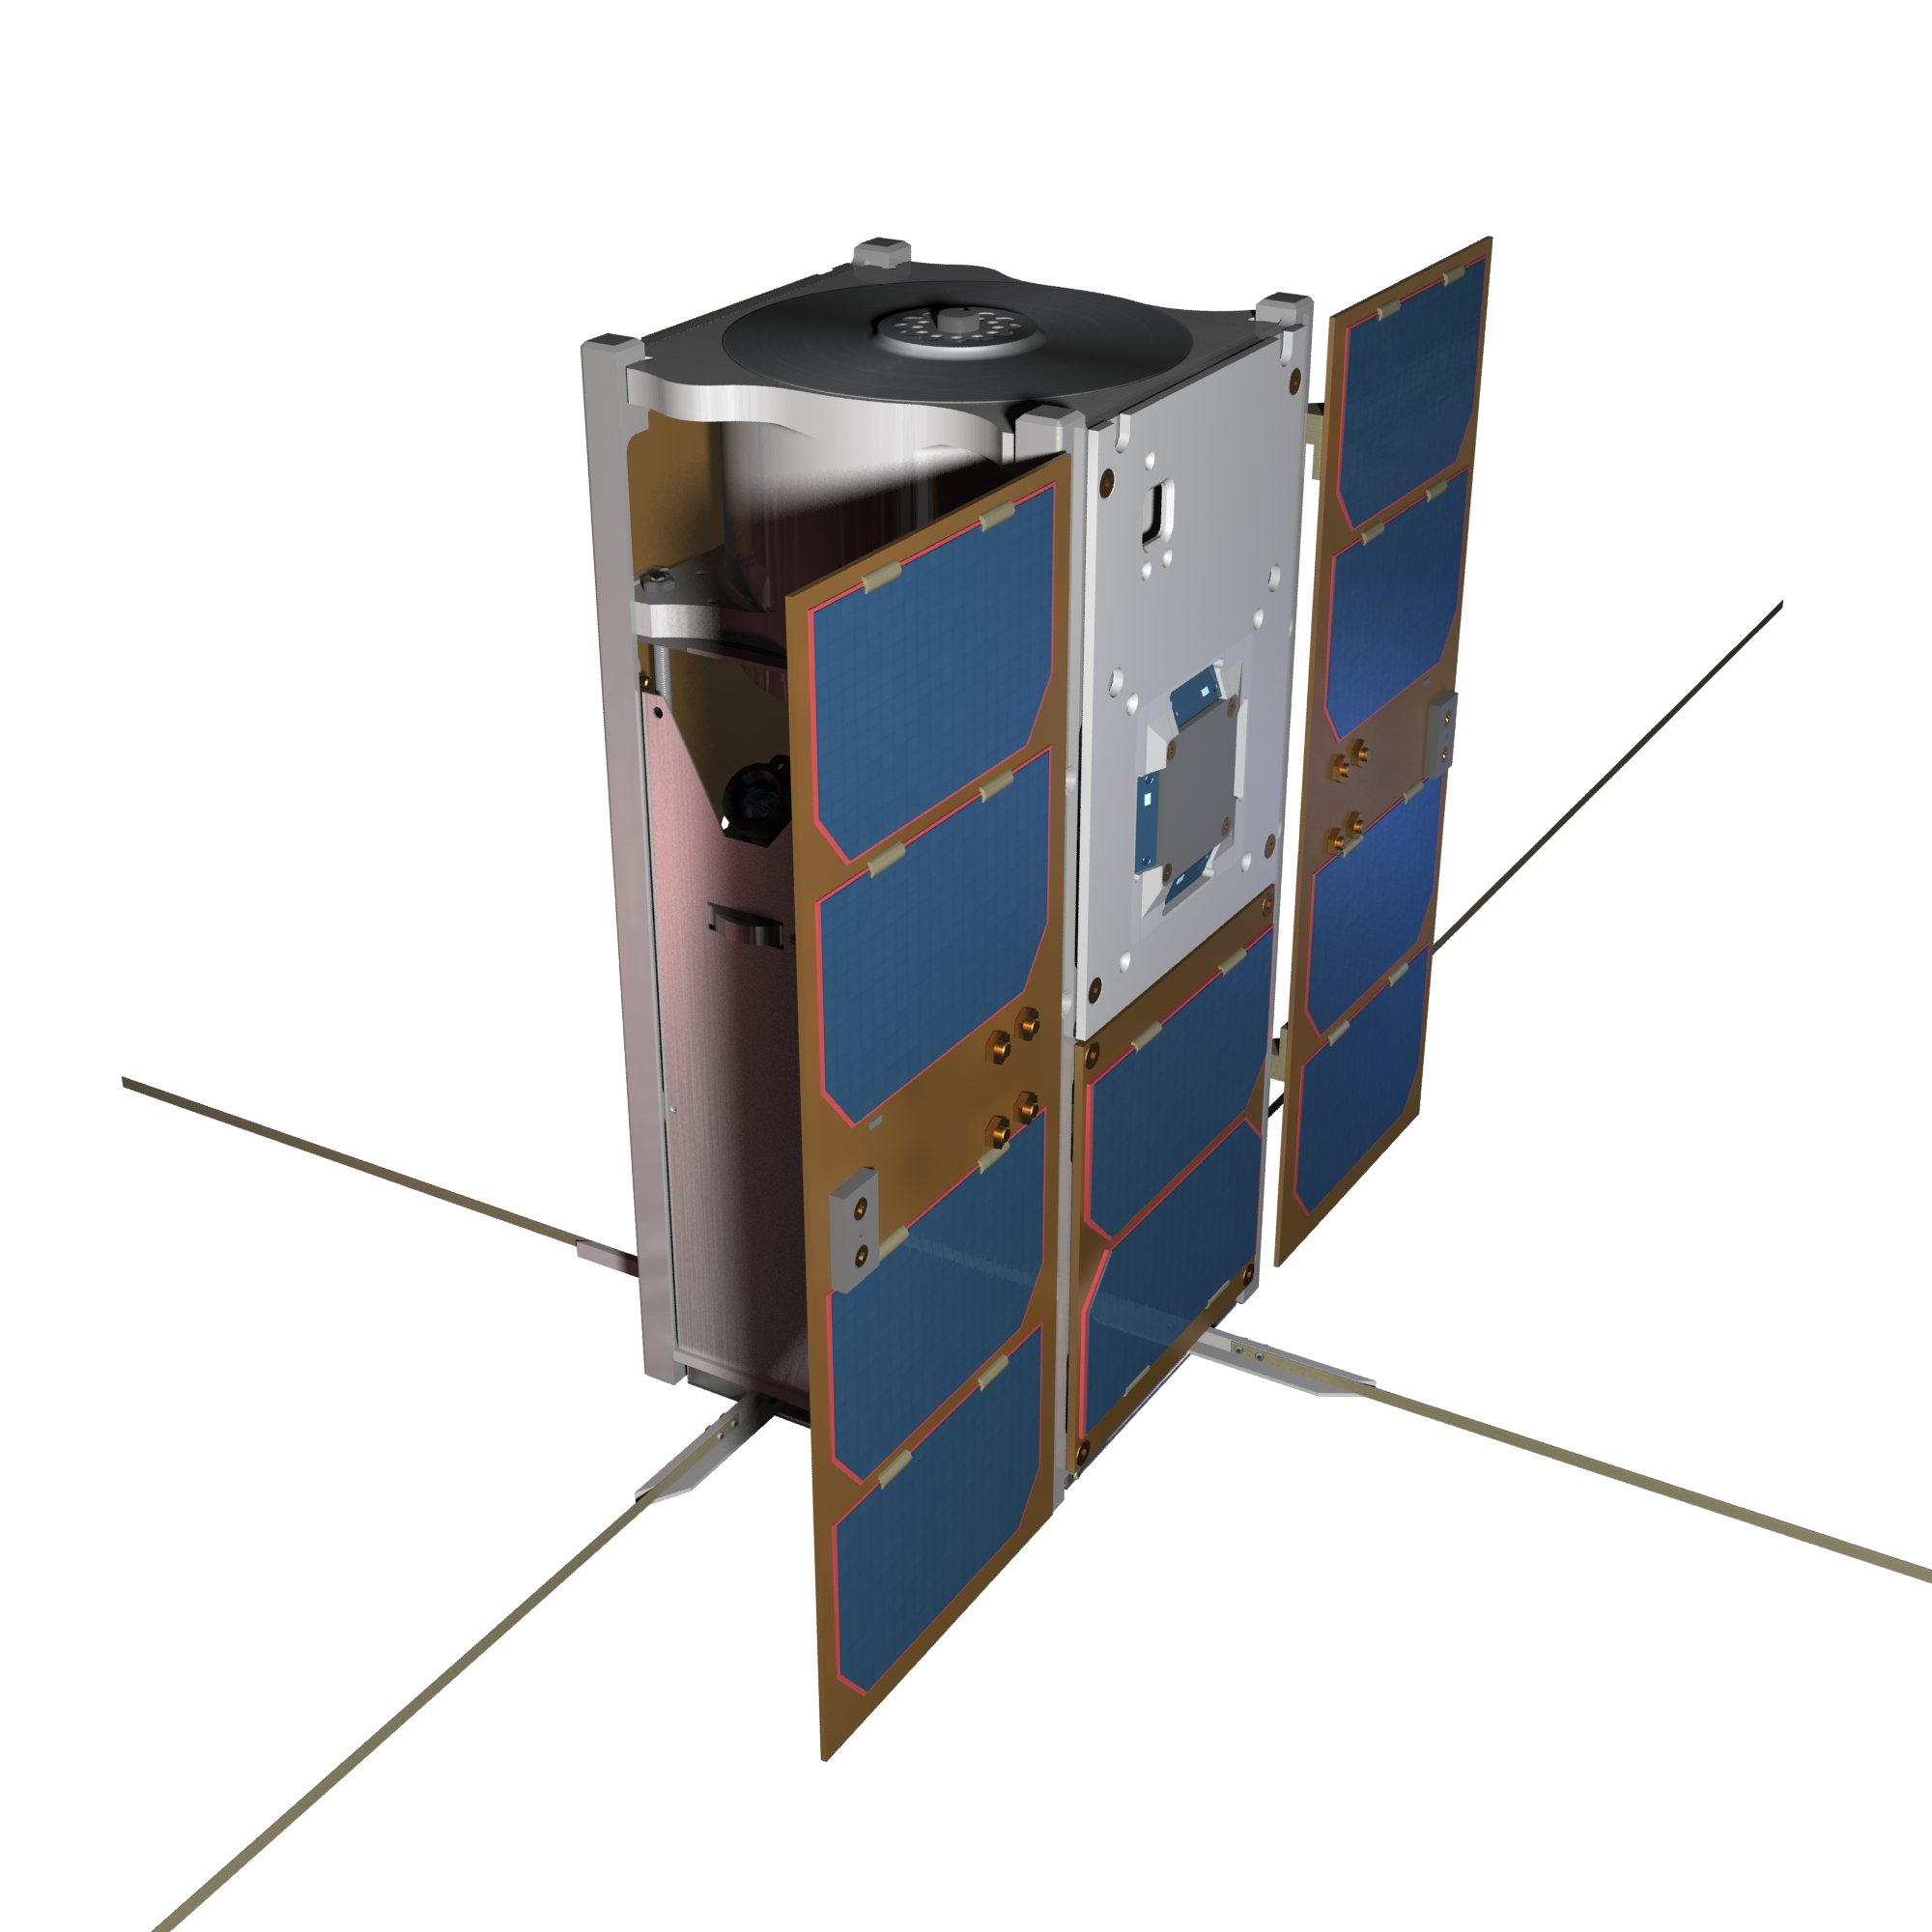
\includegraphics[width=0.5\textwidth]{PW-Sat2_2016_16_MSwietlik.png}\label{fig:pw-sat2}}
  \hfill
  \subfloat[BRITE-PL (Lem, Heweliusz)\cite{brite-pl-gunter}]
{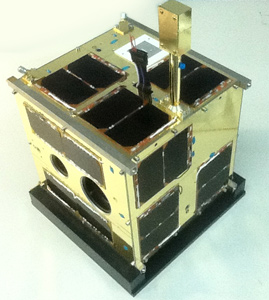
\includegraphics[width=0.5\textwidth]{brite.jpg}\label{fig:brite}}
  \caption{Example of Polish CubeSats}
  \label{fig:satellites-examples}
\end{figure}


\begin{figure}[!htbp]
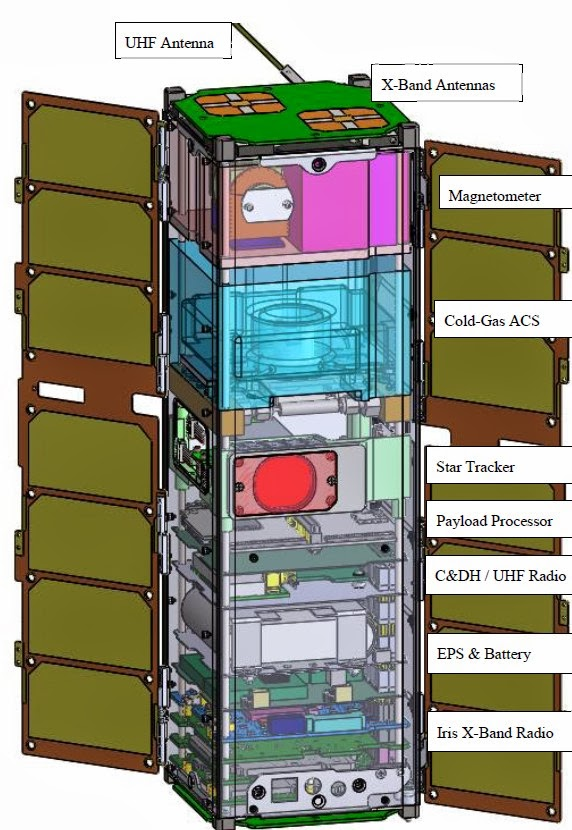
\includegraphics[scale=0.45]{INSPIRE_JPL.jpg}
\centering
\caption[CubeSat build - INSPIRE]{CubeSat build - INSPIRE, Image\cite{cubesat-build}}
\label{fig:cubesat-build}
\end{figure}

Costs of such CubeSat satellite on example of PW-SAT 2: 120,000-200,000 EUR for putting the satellite on the orbit and around 70,000 EUR for designing and building the satellite itself\cite{pw-pw-sat2}.

Another platform for slightly larger than CubeSat satellites was designed by Polish company Creotech - HyperSat\cite{hypersat}. It is based on experiences of CubeSat: it is also modular and universal. In the smallest configuration satellite can have dimensions of 30x30x10 cm and weight od 10 kg, while at largest it can have 30x30x60 cm and weight 60 kg. Because of the larger size and weight HyperSat can have more applications than CubeSat, however also lowering the price of satellite design and construction due to the standardization. The first HyperSats can enter the orbit even as soon as in 2020\cite{hypersat-space24}. The HyperSat plan considers to start serial manufacture where platform would be already prepared and configured in 6 months after ordering it\cite{platforma-satelitarna-space24}. Figure \ref{fig:hypersat-examples} shows example and prototype of HyperSat.


\begin{figure}[!htbp]
  \centering
  \subfloat[HyperSat example\cite{hypersat}]{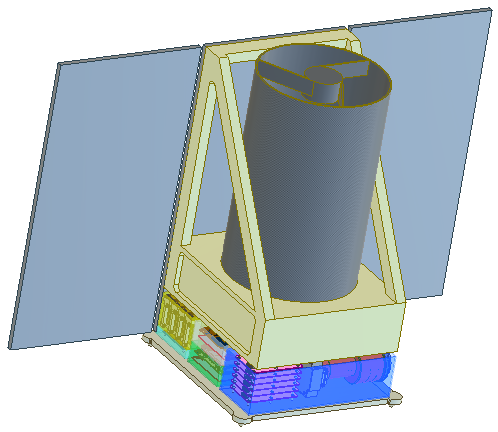
\includegraphics[width=0.4\textwidth]{Renesans_008.png}\label{fig:hypersat-concept-full}}
  \hfill
  \subfloat[HyperSat example\cite{hypersat}]{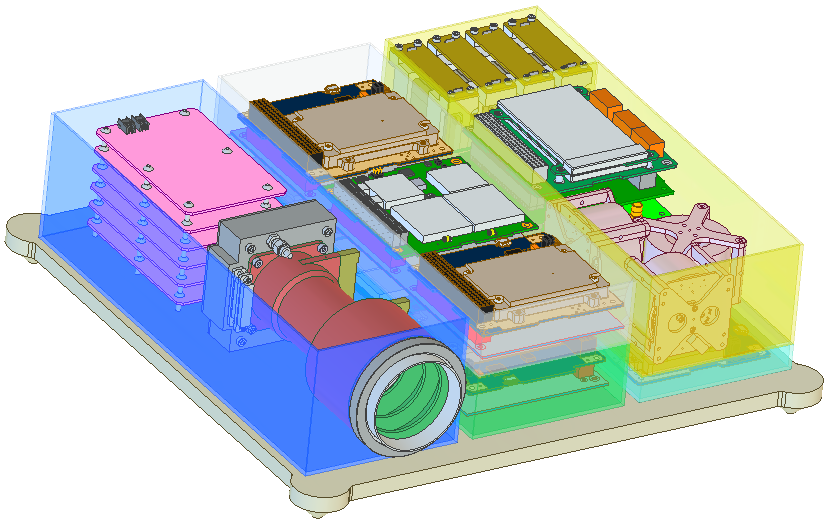
\includegraphics[width=0.6\textwidth]{Renesans_010.png}\label{fig:hypersat-concept-inside}}
  \hfill
  \subfloat[HyperSat prototype\cite{hypersat}]
{\includegraphics[width=0.7\textwidth]{hypersat_3.jpg}\label{fig:hypersat-prototype}}
  \caption{HyperSat}
  \label{fig:hypersat-examples}
\end{figure}

\subsection{Means of attitude determination}

Attitude of spaceships must be usually stabilized and controlled for various reasons.
It is necessary for satellite antenna to be pointing towards Earth for the proper communication, to intelligently control the heat by using the effects of cooling and heating of the shadows and sunlight, as well as to navigate: maneuvers must be performed in the right direction.

Attitude is determined between two coordinate systems (where one is reference system) and defines by what angles the coordinate system connected with the researched object has to be shifted in order to cover the reference system.
Devices such as planes and satellites have so called \gls{adcs}, which controls attitude of object relative to an inertial reference frame or another entity (the celestial sphere, certain areas, the nearby objects, etc.).

Currently, attitude determination of CubeSats is limited mainly to the sun sensors, magnetometers and measurements of inertia. The following table describes the accuracy of different sensors. Unquestionable winner here is the star-tracker, which, due to its quality and uniqueness of the constellations is ideal for navigation. 

\subsubsection{Inertial Measurement Unit}
An \gls{imu} detects linear acceleration using one or more accelerometers and rotational rate using gyroscopes, sometimes they also include magnetometers. They are commonly used in planes, spacecrafts and many consumer devices like smart-phones. The biggest disadvantage of \gls{imu} is accumulated error. Even small error that is accumulated with time brings device to think it is in different location than it actually is. Usually the errors are corrected via use of Kalman filter, which corrects \gls{imu} errors using other sources (i.e. \gls{gps}).
\subsubsection{Sun Sensors}
Sun sensors typically consist of few sensors oriented perpendicularly, which can tell the angle of the sun. They can give the information how the satellite is oriented towards the sun.
\subsubsection{Star-Tracker}
Star-tracker is quite sophisticated device, which consists of camera, processor and memory for database. In the database is catalog of stars, built basing on data from Earth's observatories. Simply put star-tracker, when in orbit, takes picture of space - stars. Then processes the image to recognize stars in it and compares with data in catalog or with previous image. When stars are identified star-tracker estimates the attitude of satellite towards Earth. The main advantage over other means: great accuracy and star-tracker can find its location again after satellite was restarted or lost in space.
\subsubsection{Horizon Sensors}
Earth horizon sensors use infra-red radiation from the Earth's surface via use of bolometer. The device detects when infra-red signal was first detected and then lost. The time between is used to determine the Earth's width, what later can be used to determine roll angle. In other words device detects the contrast between the cold of deep space and the heat of Earth's atmosphere. Problems of this sensors are the fact that Earth is not perfectly circular and sensors detect infra-red in the atmosphere, which varies depending on the latitude.
\subsubsection{Magnetometer}
The device actually consists of three magnetometers - one for measuring Earth's magnetic field in each direction. Measurements can be compared with known magnetic field given by International Geomagnetic Reference Field model. The problem with this sensors is that they are susceptible to noise and outside of Earth's orbit it is completely unpredictable.
\subsubsection{Global Navigation Satellite System (GNSS)}
Nowadays nearly everyone has personal device with \gls{gnss}. They are more commonly known by their implementation by various countries: \gls{gps} by USA, GLONASS by Russia, Galileo by European Union, and in close future BeiDou by China. It is possible to use \gls{gnss} to determine spacecraft's attitude. This is possible when at least four \gls{gnss} satellites are visible by spacecraft, what provides three-dimensional position. Even though it gives quite good accuracy, but it decreases with the altitude. \gls{gps} satellites are located on \gls{meo}, around 20,200 km above sea\cite{gps-gov}. It is possible to navigate spacecraft between \gls{leo} (160 to 2,000 km) and \gls{geo} (35,786 km)\cite{nasa-gps-navigation}. For missions beyond Earth's orbit \gls{gnss} navigation is however not useful. Example of \gls{gnss} usage for navigation in space is International Space Station (ISS), which uses \gls{gps}.\cite{iss-gps} There are however works that claim it could make using \gls{gps} systems possible for attitude determination up to Moon attitude in the future\cite{capuano2014gnss}.

\subsubsection{Conclusions}
The above means of attitude determination are usually used together with the use of Kalman filter, to compensate errors of one sensor with the other. However none of the means is more accurate than star-trackers.
Sun sensors can provide very accurate measurements, but can only operate in sunlight. For low-Earth orbit (LEO), even 30\% of the orbit can be done in the darkness. Magnetometers are small and can give accurate measurements if properly calibrated. Their drawback is the limited knowledge of the magnetic field and electromagnetic interference due to highly integrated construction of CubeSats.
Microelectromechanical gyroscopes are small enough to fit into a CubeSats. However, they suffer from sudden movements, and could not maintain the correct measurement of the 15-minute period of the eclipse orbit LEO. GPS navigation is accurate, however only on Earth's orbit. To be truly competitive and reliable platform, CubeSats must provide the correct determination of attitude. The best way to meet this goal is via using star-trackers. The typical accuracies of different sensors are available in Table \ref{tab:sensors}.

\renewcommand{\arraystretch}{1.5}
\begin{table}[!htbp]
\centering
\begin{tabular}{|p{5cm}|p{5cm}|}
\hline 
\textbf{Sensor} & \textbf{Accuracy} (less is better) \\ 
\hline 
Inertial Measurement Unit & 0.001\degree /hr to 1\degree /hr \\ 
\hline 
Sun Sensors & 0.005\degree{} to 3\degree \\ 
\hline 
Star Sensors & 0.0003\degree{} to 0.01\degree \newline (1 arc sec to 1 arc min) \\ 
\hline 
Horizon Sensors & 0.05\degree{} (GEO) \newline 0.1\degree{} (LEO) \\ 
\hline 
Magnetometer & 1.0\degree{} (5000km alt) \newline 5.0\degree{} (200 km alt) \\ 
\hline 
\end{tabular}
\caption[Sensor Accuracy Ranges]{Sensor Accuracy Ranges. Adapted from \citet{hall2003spacecraft} and \citet{larson1992space}}
\label{tab:sensors}
\end{table}

\subsection{NVIDIA Jetson TX2}

As mentioned before, part of the thesis is to run star-tracker program on off-the-shelf device: NVIDIA Jetson TX2\cite{nvidia-jetsontx2}. Price of this device is around 479 USD\cite{jetsontx2-price} (around 1800 PLN), what in case of successful experiment would significantly lower the price of star-trackers due to usage of already available components instead of designing new hardware.

Jetson TX2 runs Linux and provides greater than 1TFLOPS of FP16 compute performance with 7.5 watts of typical energy usage. Module has dimensions of 50 mm x 87 mm, weights 85 grams, and features the following processing components: dual-core NVIDIA Denver2 + quad-core ARM Cortex-A57, 256-core Pascal GPU and 8GB LPDDR4.
High RAM, fast multi-core CPUs and GPU allow quite complex, computing-demanding calculations to be done quickly, while some parts of star-tracker program could be done parallelly. Possibly Jetson TX2 could also be used for machine learning or deep learning star-tracker solutions, as there already exist works exploring that options. Figure \ref{fig:jetson-image} shows NVIDIA Jetson TX2 and Developer kit, while Figure \ref{fig:jetson-diagram-image} shows block diagram.

Low power consumption, low weight, small dimension, low price, already available and powerful computing components make NVIDIA Jetson TX2 good candidate for possible usage on satellites.

\begin{figure}[!htbp]
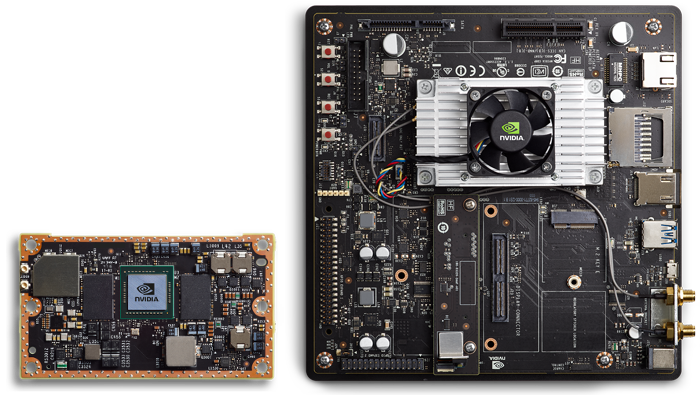
\includegraphics[angle=90, scale=0.7]{NVIDIA_Jetson_TX2_Module_Devkit.png}
\centering
\caption[NVIDIA Jetson TX2 module]{Top: Developer kit, bottom: NVIDIA Jetson TX2 module\cite{nvidia-jetsontx2}}
\label{fig:jetson-image}
\end{figure}

\begin{figure}[!htbp]
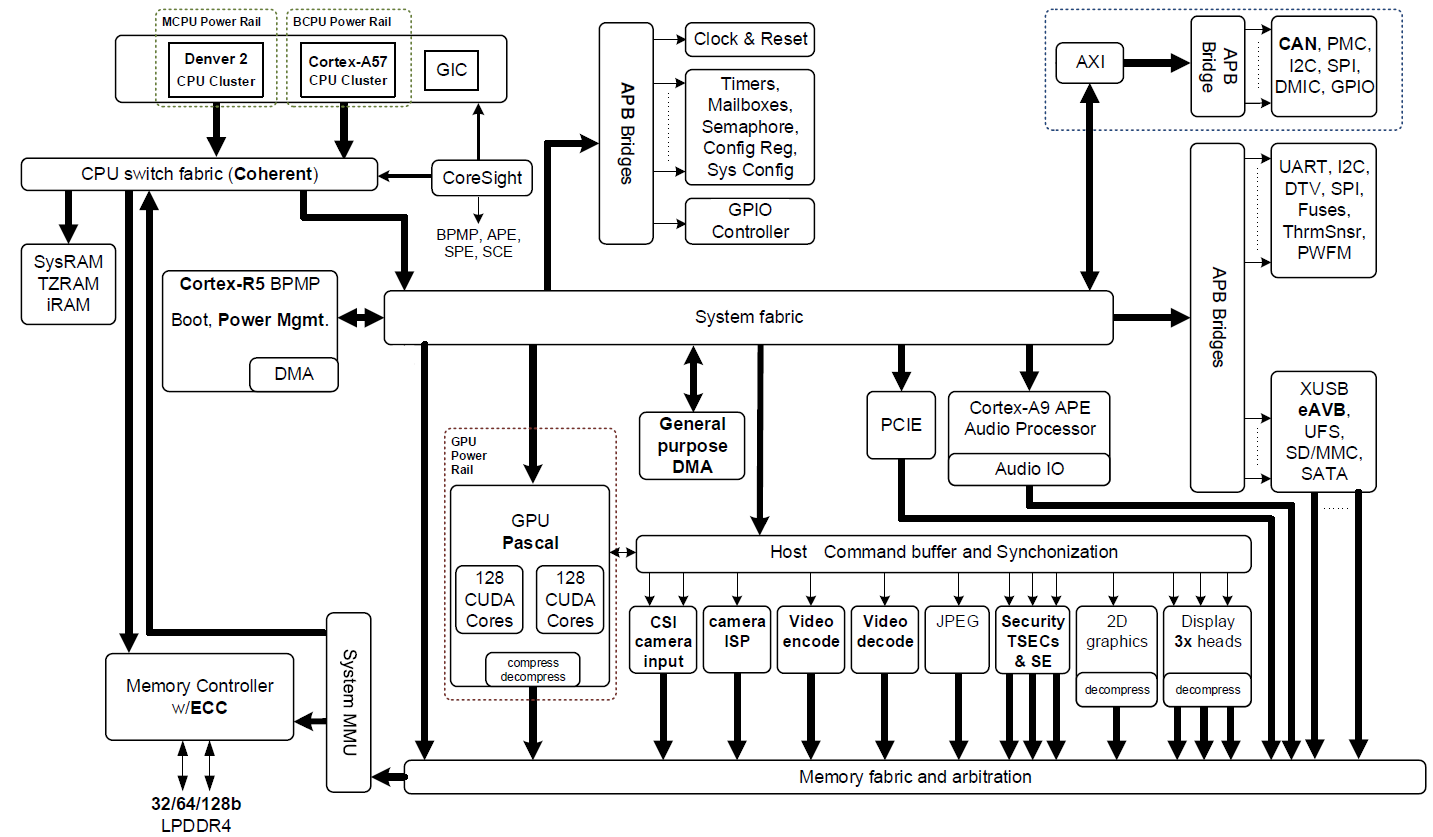
\includegraphics[angle=90, scale=0.5]{Tegra_Parker_Block_Diagram-1.png}
\centering
\caption[NVIDIA Jetson TX2 block diagram]{NVIDIA Jetson TX2 block diagram\cite{nvidia-jetsontx2}}
\label{fig:jetson-diagram-image}
\end{figure}


\cleardoublepage
\section{Preliminaries}
\subsection{Earth's orbits}

Most of spacecrafts' missions take place on Earth's orbits. There exist a variety of different classifications of orbits. Here will be presented only a few necessary to understand the topic.

Centric classification:

\begin{itemize}
\item geocentric - orbit around Earth
\item heliocentric - orbit around the Sun
\item Lunar orbit - orbit around the Earth's moon
\end{itemize}

Orbital period classification:

\begin{itemize}
\item \gls{gso} - period of rotation is equal to one sidereal day (23 hours, 56 minutes, and 4 seconds) in the same direction as Earth. This results that satellite stays in the same meridian, but can move in the North-South axis. The altitude of such orbits is 35,786 km above sea level.
\item \gls{geo} - Special case of \gls{gso}. A \gls{geo} stays exactly above the equator. For the observer on the surface the satellite stays always at the same point in the sky. Most commercial communication, broadcast and Satellite-Based Augmentation System (SBAS - system complementing GNSS) satellites use \gls{geo}s.
\item semi-synchronous - orbit has an orbital period of ½ sidereal day. The example here are orbits of \gls{gps} satellites.
\end{itemize}
\pagebreak
Altitude classification: 

\begin{itemize}
\item \gls{leo}: altitudes from 160 to 2,000 km. Used among others for ISS, Earth observation and spy satellites, some communication satellites like Iridium phones network, Hubble Space Telescope. Every object on altitude below 160 km will quickly loose it's altitude and it's orbit will decay.
\item \gls{meo}: altitudes from 2,000 km to 35,786 km. Used for navigation, communication, space environment science. Most commonly used is the altitude approximately 20,00 km, because it has orbital period of ½ sidereal day. It is used for example by GPS. Other GNSS satellites' orbits are 19,000 km for GLONASS and 23,222 km for Galileo.
\item \gls{gso} and \gls{geo} orbits - altitude approximately 35,786 km.
\item High Earth orbit: altitude above 35,786 km. Orbital periods are longer than 1 sidereal day.

\end{itemize}

The mentioned orbits are visible to some extend in the Figure \ref{fig:orbits-image}. Of course this is just a small variety of possible orbits, however describing more is not necessary for the purpose of this work.


\begin{figure}[!htbp]
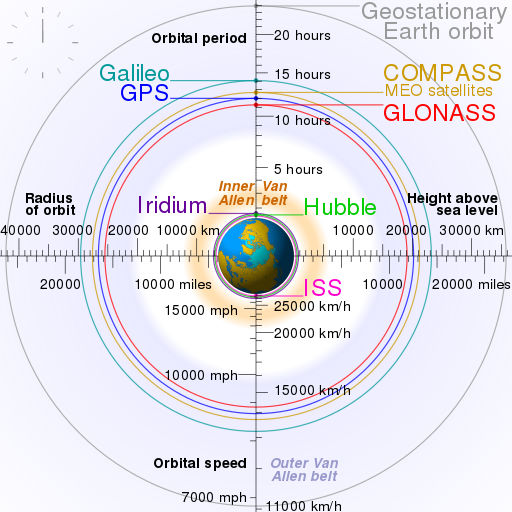
\includegraphics[scale=0.7]{Comparison_satellite_navigation_orbits.png}
\centering
\caption[Earth's satellites navigation orbits]{Earth's satellites navigation orbitsorbits-image}}
\label{fig:orbits-image}
\end{figure}


\subsection{Coordinate frames}
Describing attitude is not that simple outside Earth's surface. Earth rotates and moves around the Sun, therefore it is necessary to understand means needed for correct attitude description.
Below are described a few important frames important for understanding this work. 

\subsubsection{ECEF frame}
Earth-Centered, Earth-Fixed frame is visible in Figure \ref{fig:ecef_frame}. Its x axis points towards intersection between Greenwich Meridian and equator, while its z-axis points along the rotation axis of the Earth. The y-axis completes a right handed orthogonal coordinate system. The origin of the frame is at the center of the Earth.
This all means that the coordinates move together with Earth's rotation. It is good frame for representing objects on Earth's surface, but not for objects in space.

\begin{figure}[!htb]
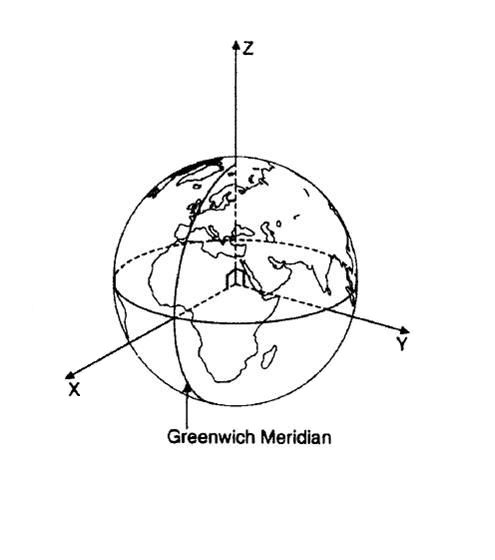
\includegraphics[scale=0.4]{eci_frame.jpg}
\centering
\caption[ECEF frame]{ECEF frame, Image from \citet{larson1992space}}
\label{fig:ecef_frame}
\end{figure}

\subsubsection{ECI frame}
The Earth Centered Inertial frame is similar to ECEF, with the difference that it is inertial - it does not follow Earth's rotation, but stays the same despite the planet's rotation. The origin of the frame is at the center of the Earth. It is much better frame for representing objects in space\cite{larson1992space}. This is the frame used in multiple catalogs, also in Hipparcos catalog used in this work.

\subsubsection{NED frame}
The North East Down frame is represented in Figure \ref{fig:ned_frame}. Its z-axis points downwards, perpendicular to the tangent plane of Earth. The x-axis points towards true north and the y-axis points East. The NED frame is an inertial frame - not dependent on Earth's rotation.

\begin{figure}[!htb]
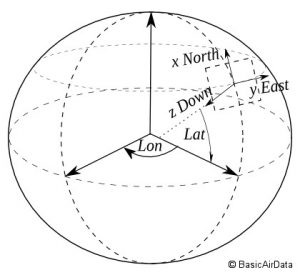
\includegraphics[scale=0.6]{ned_frame.jpg}
\centering
\caption[NED frame]{NED frame\cite{ned-frame-image}}
\label{fig:ned_frame}
\end{figure}

\subsubsection{BODY frame}
In this frame the origin is the center of the spacecraft. The moves and rotates with the spacecraft. The x-axis points forward from spacecraft, the y-axis points to the right side and the z-axis points downwards. The frame is represented in Figure \ref{fig:body_frame}. The result of the star identification is in this frame, later converted into ECI frame.

\begin{figure}[!htb]
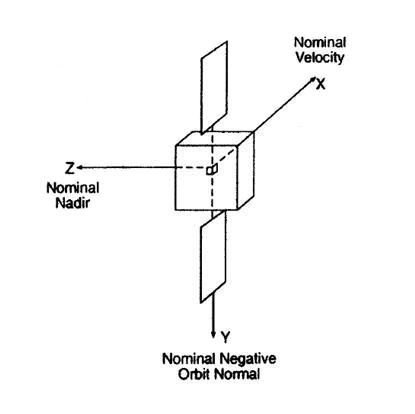
\includegraphics[scale=0.5]{body_frame.jpg}
\centering
\caption[BODY frame]{BODY frame, Image from \citet{larson1992space}}
\label{fig:body_frame}
\end{figure}

\subsection{Attitude representations}
Attitude is not only were one object is located relative to other, but also how it is rotated. It is possible to represent attitude in few ways. Here are described two most commonly used for such case: Euler angels and quaternions. Quaternions are used in all presented estimation methods.

\subsubsection{Euler angles}

Euler angles were described by Leonard Euler in 1776\cite{euler1775formulae}. They are used for representing an orientation of an object.
To fully understand the orientation between two frames it is necessary to have three parameters: one angle for the rotation around each axis. Those angles are called roll, pitch, yaw typically written as $\phi$, $\theta$ and $\psi$ respectively. The Euler angles are often used for the definition of rotation matrices about the x, y and z-axis. The equations \ref{eq:euler_rx}, \ref{eq:euler_ry} and \ref{eq:euler_rz} describe those rotation matrices.

\begin{equation} \label{eq:euler_rx}
\bm{R}_x(\phi) = \begin{bmatrix}
1 & 0 & 0 \\
0 & \cos(\phi) & -sin(\phi) \\
0 & \sin(\phi) & \cos(\phi)
\end{bmatrix}
\end{equation}
\begin{equation} \label{eq:euler_ry}
\bm{R}_y(\theta) = \begin{bmatrix}
\cos(\theta) & 0 & \sin(\theta) \\
0 & 1 & 0 \\
-\sin(\theta) & 0 & \cos(\theta)
\end{bmatrix}
\end{equation}
\begin{equation} \label{eq:euler_rz}
\bm{R}_z(\psi) = \begin{bmatrix}
\cos(\psi) & -\sin(\psi) & 0 \\
\sin(\psi) & \cos(\psi) & 0 \\
0 & 0 & 1
\end{bmatrix}
\end{equation}

\subsubsection{Quaternions}

In 1843 Sir William Rowan Hamilton described quaterions\cite{hamilton1844lxxviii} and in 1845 multiplication of quaternions to describe rotations were published by Arthur Cayley\cite{cayley1845xiii}. Quaternions consist of four elements: three give the coordinates and fourth describing angle of rotation \citet{courant1953methods}.
A quaternion can be described as a four-dimensional vector:
\begin{equation}
\bm{q} \coloneqq \begin{bmatrix}
q_0 \\
q_1 \\
q_2 \\
q_3
\end{bmatrix}
\end{equation}

where real part can be described using a rotation angle $v$, as follows:
\begin{equation}
q_0 = \cos(v/2)
\end{equation}

\begin{equation}
\bm{n} = \frac{\bm{n}}{||\bm{n}||}
\end{equation}
The imaginary part can be written as a vector:
\begin{equation}
\bm{q}_{vec} \coloneqq \begin{bmatrix}
q_1 \\
q_2 \\
q_3
\end{bmatrix}
= [\bm{n}\sin(v/2)]
\end{equation}
where $\bm{n} = \frac{\bm{n}}{||\bm{n}||}$.

In code the so called $x,y,z,w$ representation is used, where the scalar part is the last element of the vector:
\begin{equation} \label{eq:code_quaternion}
\bm{q} \coloneqq \begin{bmatrix}
q_1 \\
q_2 \\
q_3 \\
q_0
\end{bmatrix}
\end{equation}

\subsubsection{Advantages of quaternions}

Quaternions are easier to use in calculations, have more compact notation and errors easier to handle than in matrix representation. Also normalization of quaternions is easier and cheaper computationally than normalization of matrices.
The most important advantage of quaternions over Euler angles is being safe from gimbal lock. Gimbal lock is the loss of one degree of freedom that occurs when axes of two of three gimbals are driven into a parallel configuration. This could lead to real disaster \citet{shoemake1985animating}.

Quaternions show many advantages, and due to possible spins of satellites, quaternions are the only logical choice to be used for attitude estimation methods. However the visualization of attitude it is mostly done with Euler angles due to its intuitiveness.

\subsubsection{Wahba's problem}


In 1965 Grace Wahba posed the problem of finding the proper orthogonal matrix $A$ that minimizes the non-negative loss function\cite{wahba1965least}

\begin{equation}
L(A) = \frac{1}{2} \sum_i^n|\bm{b}_i - \bm{Ar}_i|^2
\end{equation}

where $\bm{b}_i$ are unit vectors in body frame, $\bm{r}_i$ are the corresponding unit vectors in a reference (NED) frame and $n$ is the number of observations.

If the vectors are error-free and the true attitude matrix $A_{true}$ is assumed to be the same for all the measurements, then $\bm{b}_i = A_{true}\bm{r}_i$ for each $i$ and the loss function $L(A) = 0$ for $A = A_{true}$.


\newpage
\section{Star-tracker program}

Star-tracker program is designed to determine the attitude of the satellite with the image of the stars made by the satellite camera. Before the start of the mission star catalog is generated, based on the star catalogs obtained from the observatories on Earth and uploaded to the computer on-board the satellite. 

After the start, the satellite is released from rocket's tank in space and has no idea where it is. Then the star-tracker on the satellite enters into Lost-In-Space mode (LIS) and analyses the current image of the stars of the camera, and then searches the corresponding result of stars in the on-board star catalog database. If it finds an entry in the database, the satellite goes into tracking mode. This means each next calculation of the orientation of the satellite attitude is going to be based on a comparison of the current pictures of stars with the preceding ones. If it cannot find the result in the database, this action is repeated from time to time, until a match is found in the database and the program will go into tracking mode.

Of course LIS does not happen only at the beginning of the satellite's flight, but can also result from many causes, e.g. a satellite which is for a long time in the darkness may discharge its battery, and during the next entry into sunlit zone will turn on and look again its attitude. Another case is when satellite becomes lost, although once found the orientation and follow her. This happens, because the successive results are based on preceding ones and even the smallest mistake will grow until the satellite will not be able to correctly calculate their attitude. It may also happen that the satellite will rotate around its axis so fast that the program would not keep up with the processing the image and calculations. In this case, the corresponding other satellite's systems should take an action reducing his spin, but this is not part of this work. It is showed in simple conceptual diagram - Figure \ref{fig:star-tracker_conceptual_alg}.

\begin{figure}[ht]
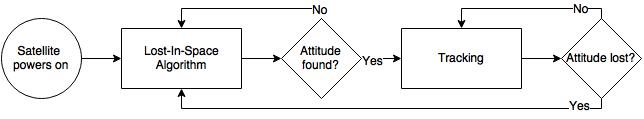
\includegraphics[scale=0.59]{startracker_eng.jpg}
\centering
\caption{Star-tracker conceptual algorithm diagram}
\label{fig:star-tracker_conceptual_alg}
\end{figure}

Each part - LIS and tracking - consists of smaller algorithms. Lost-In-Space at the beginning of reading an image from the camera, thresholds the image. Thresholding is basically throwing away parts of the image which do not exceed the threshold brightness, making just bright enough stars taken into account. Next it calculates centroid (center of mass) of selected stars, identifies these stars using one of the possible methods (here Planar Triangle, described later) and searches the directory on-board technology (k-vector).
If the database does not contain corresponding stars, the algorithm returns to the input state and starts analyzing the next image. If it manages to find the corresponding stars, the program determines the attitude of the satellite (by what angle is satellite shifted comparing to the referenced object - Earth or previous image) and enters tracking mode. Tracking mode is in large part similar to the LIS. The algorithm also first analyses the photo, selects and calculates centroids stars, identifies them, but does not search for stars in the directory board. In this algorithm are compared two images, one following after the other, and on this basis the current attitude is calculated.

Generally star-tracker is divided into three main parts\cite{mcbryde2012star}:
\begin{itemize}
\item recognizing stars on the image and converting the data into list of star vectors by calculating star centroids;
\item identifying which star vector represents which real star in catalog. This is done by comparing star vectors from the image with data in star catalog, which is generated before space mission;
\item estimating the attitude by calculating the displacement between two frames.
\end{itemize}

\subsection{Centroid - star recognition}

The whole star-tracker program is based on very precise calculations. For this reason, the calculation based on the position of the pixels only can give incorrect results. It is necessary to calculate the position of stars with an accuracy exceeding pixels. This is why the calculation of the star centroids is necessary.

The first step is the determination of stars' position in the plane of the image. If focused star pictures are recorded, the image of each star will fall only on one or two pixels, and most likely the saturate these pixels, resulting in a pixel level accuracy.
Many star-trackers are doing deliberately blurred images, in order to spread the photons on a larger number of pixels, which allows the algorithm for calculating the centroid in sub-pixel accuracy.

After the registration of such image, the centroid of the star is found similarly to the centroid weight points array, with a few differences. Firstly, instead of weight light intensity is used. Secondly, the intensity of light is usually normalized by the pixels around the star in order to filter out glare or noise. The resulting outcome is a series of two-dimensional coordinates on the photo plane with the starting point at the center of the image. This allows the system to the coordinates of the stars can be easily converted into unit vectors in the next step.

The algorithm requires specification of the light intensity threshold (to select the brightest stars) $I_{thresh}$ and the size of the Region of Interest (ROI) $a_{ROI}$ in pixels. These values are adjusted to manipulate the performance of the algorithm. For example, the higher the value of $I_{thresh}$ is more resistant to noise, but can miss some real stars in the picture. Similarly, a large value $a_{ROI}$ means a more exact value of centroid, but the algorithm can see one star there, where are actually two within a short distance of each other. The centroiding part is about trade-off between noise resistance and star recognition, and also between recognizing few close stars as one and recognizing one big star as a few.
Please note that $a_{ROI}$ must be a positive odd number for the proper functioning of the algorithm.


The idea of how to calculate such centroids is adapted from \citet{mcbryde2012star} and described below:

\begin{enumerate}
\item For each pixel at image coordinates $(x,y)$ it is checked if:
\begin{enumerate}
\item light intensity is high enough: $I(x,y) > I_{thresh}$, hence only bright points of image are taken into account;
\item the sum of light intensity of given amount of pixels around the pixel is high enough (Equation \ref{eq:centroid_magnitude}), hence only low magnitude stars are taken into account. Describing the equation: it is the pixel intensity sum of vertical, horizontal and both diagonals of pixels around the given pixel, where $lp$ is limit of pixels for magnitude ROI and $I_{thresh_{mag}}$ is limit threshold of star magnitude pixels intensity.
\begin{equation}
\begin{gathered}
\sum_{i=x-lp}^{x+lp} I(x_i,y) +  \\ 
\sum_{j=y-lp}^{y+lp} I(x,y_j) +  \\ 
\sum_{i=x-lp}^{x+lp}\sum_{j=y-lp}^{y+lp} I(x_i,y_j) +  \\ 
\sum_{i=x-lp}^{x+lp}\sum_{j=y+lp}^{y-lp} I(x_i,y_j) \\ 
> I_{thresh_{mag}}
\end{gathered}
\label{eq:centroid_magnitude}
\end{equation}

\end{enumerate}
If both above conditions are met, the algorithm moves forward. Otherwise the pixel is discarded and algorithm moves to another pixel.
In case of success, the ROI for given pixel is defined as the square of pixels with side length $a_{ROI}$ and bottom-left corner at $(x_{start},y_{start})$
\begin{equation}
x_{start} = x - \frac{a_{ROI} - 1}{2}
\end{equation}
\begin{equation}
y_{start} = y - \frac{a_{ROI} - 1}{2}
\end{equation}
\begin{equation}
x_{end} = x_{start} + a_{ROI}
\end{equation}
\begin{equation}
y_{end} = y_{start} + a_{ROI}
\end{equation}
\item If $x_{start} < 0$ or $y_{start} < 0$, discard the pixel and return to previous step with the next pixel.

\item Find the average intensity value of the border pixels
$I_{border}$
\begin{subequations}
\begin{equation}
I_{bottom} = \sum_{i=1}^{x_{end}-1} I(i, y_{start})
\end{equation}
\begin{equation}
I_{top} = \sum_{i=2}^{x_{end}} I(i, y_{end})
\end{equation}
\begin{equation}
I_{left} = \sum_{j=1}^{y_{end}-1} I(x_{start}, j)
\end{equation}
\begin{equation}
I_{right} = \sum_{j=2}^{y_{end}} I(x_{start}, j)
\end{equation}
\begin{equation}
I_{border} = \frac{I_{top} + I_{bottom} + I_{left} + I_{right}}{4(a_{ROI} - 1)}
\end{equation}
\end{subequations}

\item Normalize all the non-boarder pixels, yielding normalized light intensity matrix $\tilde{I}$

\begin{equation}
\tilde{I}(x,y) = I(x,y) - I_{border}
\end{equation}

\item Calculate centroid locations $(x_{CM}, y_{CM})$ and brightness $B$
\begin{equation}
B = \sum_{i=x_{start}+1}^{x_{end}-1}\sum_{j=y_{start}+1}^{y_{end}-1}\tilde{I}(i,j)
\end{equation}
\begin{equation}
x_{CM} = \sum_{i=x_{start}+1}^{x_{end}-1}\sum_{j=y_{start}+1}^{y_{end}-1}\frac{i \times \tilde{I}(i,j)}{B}
\end{equation}
\begin{equation}
x_{CM} = \sum_{i=x_{start}+1}^{x_{end}-1}\sum_{j=y_{start}+1}^{y_{end}-1}\frac{j \times \tilde{I}(i,j)}{B}
\end{equation}

\item When the centroid location has been calculated for each pixel above the intensity threshold, it is still necessary to make clustering of them. This is done via averaging together all values that are clustered together. Before clustering it is sure that some stars will have more centroids than one, and clustering helps merge them into one. It is configurable by the number of proximity pixels of the centroids. Of course it is not possible to do it perfectly. The main problem is that sometimes there are few stars in close proximity to each other on the photo and it is possible to count those few stars as one, while doing this correctly for all other stars in the photo. On the other hand, if threshold is lowered too much, it is possible to count few stars correctly, but also possible to count one star as a few. The Figure \ref{fig:centroids-examples} shows example of such trade-off.
The clustering can be accomplished by checking each new centroid against a list of already processed centroids. If the new location is within the given range (for example 5 pixels) it is assumed they represent the same star and therefore they values are averaged. The output of this step is the list of star centroids, where each centroid should represent separate star.


\item Now convert each found centroid location into unit vector $\bm{u}$ using the camera pixel size $\mu$ and camera focal length $f$

\begin{equation}
\bm{u} = \frac{
\begin{bmatrix}
\mu x_{CM} & \mu y_{CM} & f
\end{bmatrix}
^T}
{||
\begin{bmatrix}
\mu x_{CM} & \mu y_{CM} & f
\end{bmatrix}
||}
\end{equation}
\end{enumerate}

\begin{figure}[!htbp]
  \centering
  \subfloat[Original image]{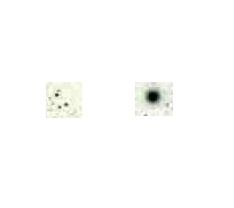
\includegraphics[width=0.5\textwidth]{centroids_1.jpg}\label{fig:centroids_1}}
  \hfill
  \subfloat[Too high pixel proximity threshold]{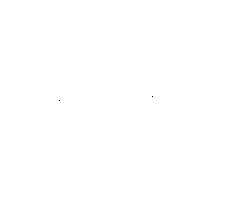
\includegraphics[width=0.5\textwidth]{centroids_2.png}\label{fig:centroids_2}}
  \hfill
  \subfloat[Too low pixel proximity threshold]{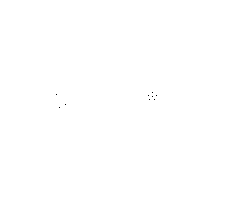
\includegraphics[width=0.5\textwidth]{centroids_3.png}\label{fig:centroids_3}}
  \hfill
  \subfloat[Ideal result of clustering]
{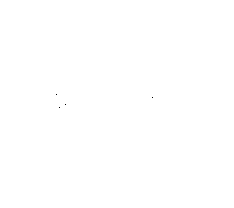
\includegraphics[width=0.5\textwidth]{centroids_4.png}\label{fig:centroids_4}}
  \caption[Example of centroids' clustering trade-off]{Example of centroids' clustering trade-off (in negative colours)}
  \label{fig:centroids-examples}
\end{figure}

\subsection{Star identification}

Star identification is the part of star-tracker program, which actually finds out which recognized stars are which. Prior this part it is only known that some stars were read from the image, and now it is the time to identify them by comparing to the on-board star catalogue. There is a number of techniques to do that\cite{spratling2009survey}. In this section most of them will be described.


\subsubsection{Angle Matching}
The Angle Matching is probably the oldest way for identifying stars. It needs at least two stars as an input\cite{gottlieb1978star}. The Figure \ref{fig:angle_matching} visualizes the way the method works.

\begin{figure}[ht]
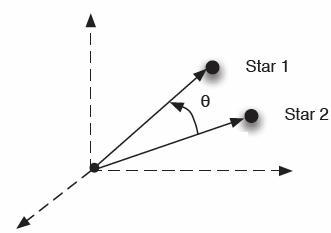
\includegraphics[scale=0.7]{vector_angle_method.jpg}
\centering
\caption[Vector angle method]{Vector angle method, Image from \citet{gottlieb1978star}}
\label{fig:angle_matching}
\end{figure}

The angle between two vectors pointing to the stars is given by:

\begin{equation}
\theta = \cos^{-1}(\bm{r}_1 \cdot \bm{r}_2)
\end{equation}
where $\bm{r}_1$ and $\bm{r}_2$ are unit vectors pointing to each star. The vectors are given in inertial space. The angle $\theta$ is the same when inertial vectors or body vectors are used. The problem is that the angle measured between stars in the image contain significant measurement error, that cannot be ignored.
What is needed by this technique, is the standard deviation of the angle between two stars when each star measurement possesses the error described. It can be used to provide a bound on the expected errors.
Firstly standard coordinate transformation is necessary:
\begin{equation}
\bm{b}_i = A\bm{r}_i
\end{equation}
where $\bm{r}_i$ is direction the direction of star in the ECI coordinate system, $A$ is the direction cosine matrix, $\bm{b}_i$ is direction of star in the star-tracker body coordinate system.

Nearly all the probability of errors is focused on a very small area about the direction of $A\bm{r}_i$, that the sphere containing that point can be approximated by a tangent plane, characterized by:
\begin{equation}
\tilde{\bm{b}}_i = A\bm{r}_i + \bm{v}_i, \hspace{0.5cm} \bm{v}_i^TA\bm{r}_i = 0
\end{equation}
where $\tilde{\bm{b}}_i$ is the it{i}th measurement and sensor $\bm{v}_i$ is approximately Gaussian, which satisfies
\begin{subequations}
\begin{equation}
E\left\{\bm{v}_i\right\} = 0
\end{equation}
\begin{equation}
E\left\{\bm{v}_i\bm{v}_i^T\right\} = \sigma_i^2 [\bm{I} - (A\bm{r}_i)(A\bm{r}_i)^T]
\end{equation}
\end{subequations}
where $\sigma_i^2$ is the variance and $E$ is expectation.
The dot product of two body observations gives
\begin{equation}
\bm{b}_1^T\bm{b}_2 = \bm{r}_1^TA^TA\bm{r}_2 = \bm{r}_1^T\bm{r}_2
\end{equation}
what show that the dot product is attitude-invariant measurement.
In case of two measurements $\bm{b}_1$ and $\bm{b}_2$ with noise, where $\bm{v}_1$ and $\bm{v}_2$ are uncorrelated:
\begin{subequations}
\begin{align*}
\tilde{\bm{b}}_1 = A\bm{r}_1 + \bm{v}_1\\
\tilde{\bm{b}}_2 = A\bm{r}_2 + \bm{v}_2
\end{align*}
\end{subequations}
define the effective measurement:
\begin{equation}
z \equiv \tilde{\bm{b}}_1^T\tilde{\bm{b}}_2 = \bm{r}_1^T\bm{r}_2 + \bm{r}_1^TA^T\bm{v}_J + \bm{r}_2^TA^T\bm{v}_1 + \bm{v}_1^T\bm{v}_2
\end{equation}
As $\bm{v}_1$ and $\bm{v}_2$ are uncorrelated, then:
\begin{equation}
E\left\{z\right\} = \bm{r}_1^T\bm{r}_2
\end{equation}
Define the following variable:
\begin{equation}
p \equiv z - E\left\{z\right\} = \bm{r}_1^TA^T\bm{v}_J + \bm{r}_2^TA^T\bm{v}_1 + \bm{v}_1^T\bm{v}_1
\end{equation}
Taking $E\left\{p^2\right\}$ gives the variance for the dot product measurement error:
\begin{equation}
\begin{split}
\sigma_p^2 \equiv E\left\{p^2\right\} = \\
\bm{r}_1^TA^TR_2A\bm{r}_1 + \bm{r}_2^TA^TR_aA\bm{r}_2 + Trace(R_1R_2) = \\
Trace(A\bm{r}_1\bm{r}_1^TR_2) + Trace(A\bm{r}_2\bm{r}_2^TR_1) + Trace(R_1R_2)
\end{split}
\end{equation}
where $E\left\{\bm{v}_1\bm{v}_1^T\right\}\equiv R_1$ and $E\left\{\bm{v}_2\bm{v}_2^T\right\}\equiv R_2$.

The effective measurement noise in the dot product consist of both Gaussian and chi-squared distribution, but since the noise is small in comparison to the unit vector observation, the effective noise can be treated as purely Gaussian. As the attitude is not known, the $A\bm{r}_1$ and $A\bm{r}_2$ are replaced by $\tilde{\bm{b}}_1$ and $\tilde{\bm{b}}_2$. Errors introduced in this substitution are second-order in nature, hence the variance is completely independent of the attribute matrix $A$.

In case there exist more than one possible solution, so called pivoting is made. This means that if for first angle more than one solution was found, the second angle is selected, that shares one common star with the first angle. When all solutions for second angle are obtained, the solutions not common for those two angles are discarded. If there is still more than one solution, then another pivot is made. Now it compares the second angle with third angle, with a common star. The rest goes analogically. This happens till finally there is only one solution for some two angles, or there are no more angles left in the input, and system enters into LIS mode.

\subsubsection{Spherical Triangle Matching}

Instead of measuring the inter-star angle, this method creates spherical triangles out of three stars. Due to that more information can be obtained from such triangle than an angle, what enables to identify stars faster and using fewer stars overall than in previous method. In this technique the area and polar moment are used instead of angles. The main disadvantage comparing to angle matching method is that this one requires not two but three stars in order to work properly, however under typical conditions in angle matching it is necessary to use more stars due to measurement error. Also the spherical triangle catalogue is about 10 times larger than angle catalogue\cite{cole2004fast}.

\begin{figure}[ht]
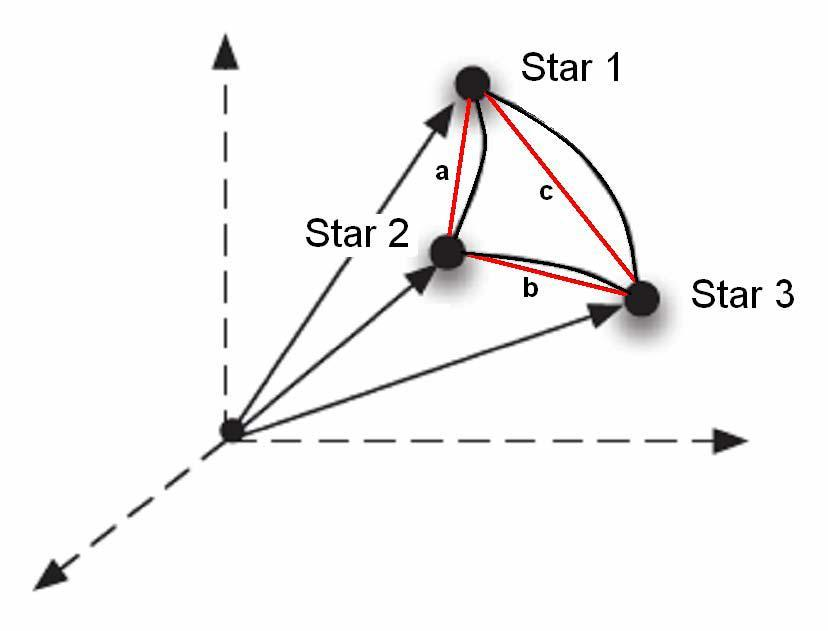
\includegraphics[scale=0.29]{spherical_triangle_method.jpg}
\centering
\caption[Spherical Triangle Method]{Spherical Triangle Method, Image from \citet{cole2004fast}}
\label{fig:spherical_triangle_method}
\end{figure}
Given three unit vectors pointing toward three stars, the area of a spherical triangle is as follows:
\begin{equation}
A = 4\tan^{-1}\sqrt{\tan\frac{s}{2}\tan\frac{s-a}{2}\tan\frac{s-b}{2}\tan\frac{s-c}{2}}
\end{equation}
where
\begin{subequations}
\begin{align*}
s = \frac{1}{2}(a + b + c) \\
a = \cos^{-1} \bigg(\frac{\bm{b}_1 \cdot \bm{b}_2}{|\bm{b}_1||\bm{b}_2|}\bigg) \\
b = \cos^{-1} \bigg(\frac{\bm{b}_2 \cdot \bm{b}_3}{|\bm{b}_2||\bm{b}_3|}\bigg) \\
c = \cos^{-1} \bigg(\frac{\bm{b}_3 \cdot \bm{b}_1}{|\bm{b}_3||\bm{b}_1|}\bigg) 
\end{align*}
\end{subequations}
The equation is given for the body frame, but can be used in the ECI frame too. To get a bound for the measurement error, the standard deviation must be calculated.

The polar moment is good supplement to area, because it is possible for two spherical triangles to have the same area but different polar moment, and all way around. This helps to quickly reduce the number of possible solutions.

The polar moment can be obtained as follows
\begin{equation}
I_p = \sum\theta^2dA
\end{equation}

The polar moment of each spherical triangle is calculated by recursive algorithm, which divides the triangle into smaller triangles till the recursion's depth is met.

The standard deviations for area and polar moment are given by \citet{cole2004fast}.

In this technique pivoting works analogically to the angle matching method. Note that while calculation of the standard deviation of area is quite straightforward, the standard deviation of the second moment calculation is difficult to compute analytically.

\subsubsection{Planar Triangle}

The third technique, quite similar to previous one is Planar Triangle. Instead of spheres it uses planes, what makes it much less computationally demanding. It also uses the same two properties: triangle area and polar moment. In this case also three stars are necessary\cite{cole2006fast}.

\begin{figure}[ht]
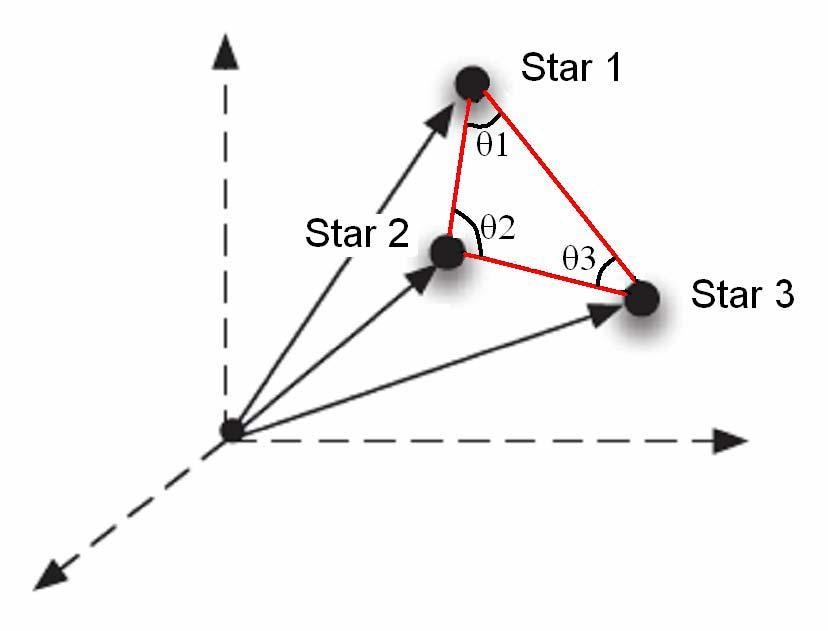
\includegraphics[scale=0.30]{planar_triangle_method.jpg}
\centering
\caption[Planar Triangle Method]{Planar Triangle Method, Image from \citet{cole2006fast}}
\label{fig:planar_triangle_method}
\end{figure}

Given thee unit vectors pointing toward three stars $\bm{u_p}$, $\bm{u_q}$, $\bm{u_r}$, the area for planar triangle is as follows:
\begin{equation}
A = \sqrt{s(s-a)(s-b)(s-c)}
\end{equation}
where
\begin{subequations}
\begin{equation}
s = \frac{1}{2}(a + b + c)
\end{equation}
\begin{equation}
a = ||\bm{u_p} - \bm{u_q}||
\end{equation}
\begin{equation}
b = ||\bm{u_q} - \bm{u_r}||
\end{equation}
\begin{equation}
c = ||\bm{u_p} - \bm{u_r}||
\end{equation}
\end{subequations}

The equation is given for the body frame, similarly as for the spherical triangle. It can be also used for ECI frame. Also here the standard deviation has to be calculated in order to obtain a bound of the measurement error.

Similarly as in the previous method, here also polar moment is calculated:
\begin{equation}
J = A\frac{(a^2 + b^2 + c^2)}{36}
\end{equation}

Since the planar area is a nonlinear function, a linearization must be used to determine its variance. To compute this, the following matrix must be evaluated:

Derivatives
\begin{equation}
H = \begin{bmatrix}
\bm{h}_1^T & \bm{h}_2^T & \bm{h}_3^T
\end{bmatrix}
\end{equation}
where
\begin{subequations}
\begin{equation}
\bm{h}_1^T \equiv \frac{\delta A}{\delta a}\frac{\delta a}{\delta\bm{b}_1} + \frac{\delta A}{\delta c}\frac{\delta c}{\delta\bm{b}_1}
\end{equation}
\begin{equation}
\bm{h}_2^T \equiv \frac{\delta A}{\delta a}\frac{\delta a}{\delta\bm{b}_2} + \frac{\delta A}{\delta b}\frac{\delta b}{\delta\bm{b}_2}
\end{equation}
\begin{equation}
\bm{h}_3^T \equiv \frac{\delta A}{\delta b}\frac{\delta b}{\delta\bm{b}_3} + \frac{\delta A}{\delta c}\frac{\delta c}{\delta\bm{b}_3} 
\end{equation}
\end{subequations}
To calculate the partials with respect to $a$, $b$ and $c$ serve the following equations:
\begin{subequations}
\begin{equation}
\frac{\delta A}{\delta a} = \frac{u_1 - u_2 + u_3 + u_4}{4A}
\end{equation}
\begin{equation}
\frac{\delta A}{\delta b} = \frac{u_1 + u_2 - u_3 + u_4}{4A}
\end{equation}
\begin{equation}
\frac{\delta A}{\delta c} = \frac{u_1 + u_2 + u_3 - u_4}{4A}
\end{equation}
\end{subequations}
where
\begin{subequations}
\begin{equation}
u_1 = (s - a)(s - b)(s - c)
\end{equation}
\begin{equation}
u_2 = s(s - b)(s - c)
\end{equation}
\begin{equation}
u_3 = s(s - a)(s - c)
\end{equation}
\begin{equation}
u_4 = s(s - a)(s - b)
\end{equation}
\end{subequations}
The partials with respect to $\bm{b}_1$, $\bm{b}_2$ and $\bm{b}_3$ are calculated formulas
\begin{subequations}
\begin{equation}
\frac{\delta a}{\delta \bm{b}_1} = (\bm{b}_1 - \bm{b}_2)^T /a, \hspace{0.5cm} \frac{\delta a}{\delta \bm{b}_2} = -\frac{\delta a}{\delta \bm{b}_1}
\end{equation}
\begin{equation}
\frac{\delta b}{\delta \bm{b}_2} = (\bm{b}_2 - \bm{b}_3)^T /b, \hspace{0.5cm} \frac{\delta b}{\delta \bm{b}_3} = -\frac{\delta b}{\delta \bm{b}_2}
\end{equation}
\begin{equation}
\frac{\delta c}{\delta \bm{b}_1} = (\bm{b}_1 - \bm{b}_3)^T /c, \hspace{0.5cm} \frac{\delta c}{\delta \bm{b}_3} = -\frac{\delta c}{\delta \bm{b}_1}
\end{equation}
\end{subequations}
The variance of the area is as follows
\begin{equation}
\sigma_A^2 = HRH^T
\end{equation}
where
\begin{equation}
R \equiv \begin{bmatrix}
R_1 & 0_{3x3} & 0_{3x3} \\
0_{3x3} & R_2 & 0_{3x3} \\
0_{3x3} & 0_{3x3} & R_3
\end{bmatrix}
\end{equation}

As with the area, it is necessary to obtain the variance of the polar moment. The following partial matrix has to be evaluated first:

\begin{equation}
\bar{H} = \begin{bmatrix}
\bar{\bm{h}}_1^T & \bar{\bm{h}}_2^T & \bar{\bm{h}}_3^T
\end{bmatrix}
\end{equation}
where
\begin{subequations}
\begin{equation}
\bar{\bm{h}}_1^T \equiv \frac{\delta J}{\delta a}\frac{\delta a}{\delta\bm{b}_1} + \frac{\delta J}{\delta c}\frac{\delta c}{\delta\bm{b}_1} + \frac{\delta J}{\delta A}\bm{h}_1^T
\end{equation}
\begin{equation}
\bar{\bm{h}}_2^T \equiv \frac{\delta J}{\delta a}\frac{\delta a}{\delta\bm{b}_2} + \frac{\delta J}{\delta b}\frac{\delta b}{\delta\bm{b}_2} + \frac{\delta J}{\delta A}\bm{h}_2^T
\end{equation}
\begin{equation}
\bar{\bm{h}}_3^T \equiv \frac{\delta J}{\delta b}\frac{\delta b}{\delta\bm{b}_3} + \frac{\delta J}{\delta c}\frac{\delta c}{\delta\bm{b}_3} + \frac{\delta J}{\delta A}\bm{h}_3^T
\end{equation}
\end{subequations}
with
\begin{subequations}
\begin{equation}
\frac{\delta J}{\delta a} = \frac{-b^3 * A * 2 * a * b^2 * A}{18 * b^2}
\end{equation} 
\begin{equation}
\frac{\delta J}{\delta b} =  \begin{multlined}
\frac{4 * b^3 * A - 3 * a * b^2 * A + 2 * a^2 * b * A}{18 * b^2} - \\ 
\frac{b^*4 * A - a * b^3 * A + a^2 * b^2 * A + 4 * A^3}{9 * b^3} \end{multlined}
\end{equation}
\begin{equation}
\frac{\delta J}{\delta c} = \frac{b^4 - a * b^3 + a^2 * b^2 + 12 * A^2}{18 * b^2}
\end{equation}
\begin{equation}
\frac{\delta J}{\delta A} = (a^2 + b^2 + c^2)/36
\end{equation}
\end{subequations}
Other quantities are given from the area variance calculations. The variance of the polar moment is calculated with the following formula:
\begin{equation}
\sigma_J^2 = \bar{H}R\bar{H}^T
\end{equation}

Pivoting works analogically as in the previous methods.

This method gives similar results as spherical triangle method, but planar triangle method does not have to perform recursive calculations of polar moment like the previous method, hence it has lower computational demand for star-identification\cite{alidoost2013review}.	


\subsubsection{Pyramid}

Pyramid method is described by \citet{mortari2004pyramid}. This algorithm is designed to be used efficiently with 4-star input, however can also function for 3-star input if no more are available. It uses set of star pairs in elementary measured star polygons (3 for a triangle, six for a 4-star pyramid). The vertices between adjacent measured star pairs share a common cataloged star.

The Figure \ref{fig:pyramid_method} shows how the algorithm works. If there are less than 3 stars on input, the algorithm returns error, what actually brings back to start of the algorithm with new input data. In case there are three stars only, algorithm gets rid of redundant solutions, and if the solution is unique, the stars are identified and solution is outputted. In case of not finding unique solution, algorithm returns an error, and starts again with new data. If there are more than three stars, algorithm gets three stars for a triangle, and then one reference star. Later it checks pairs of reference star and triangle's vertices. If unique solution is found, it identifies the remaining stars and outputs all the identified stars. If no unique solution has been found, algorithm tries to get new triangle and repeat the steps. There are two possible exits of this loop: the already mentioned finding unique solution, or running out of new triangles. In the last case algorithm removes redundant solutions, then check again if it is unique solution. Finally either unique solution is found and algorithm identifies all other stars from the input and outputs them, or returns an error and stars again with the new input data.

\begin{figure}[!htbp]
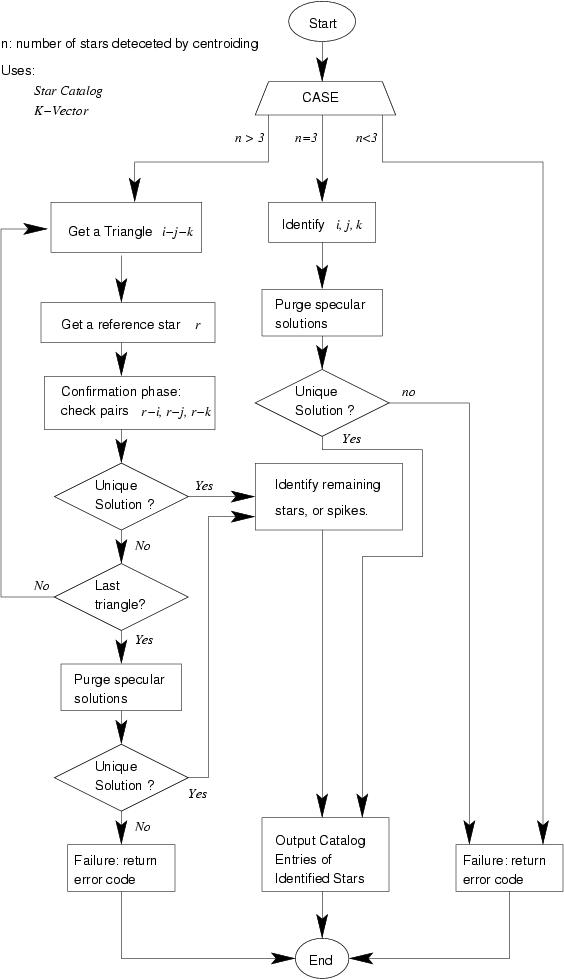
\includegraphics[scale=0.57]{pyramid_method.jpg}
\centering
\caption[Pyramid Method Flowchart]{Pyramid Method Flowchart, Image from \citet{mortari2004pyramid}}
\label{fig:pyramid_method}
\end{figure}

According to authors the algorithm can solve LIS problem and is highly robust. The key to algorithm's efficiency lies in the usage of k-vector method and the usage of expected random frequencies connected to matching interstar angles from measured star polyhedron. The algorithm has been tested on Draper’s “Inertial Stellar Compass” star tracker\cite{brady2002inertial} and on MIT’s satellites HETE and HETE-2\cite{crew2002hete} successfully. This algorithm is currently under exclusive contract to StarVision Technologies\cite{jacox2006method}\cite{pyramid-starvision}.


\subsubsection{Voting}
Algorithm was presented by \citet{kolomenkin2008geometric}. Pair of stars in the catalog votes for a pair of stars in the image if angular distance between the stars of both pairs is similar. Since angular distance is a symmetric relationship, each catalog star in the pair vote for each in the image pair. Then the image star is identified as the catalog star which gave the most votes.

Authors' testing has shown that the algorithm is as accurate, as fast and more robust than other methods. The authors tested the algorithm in simulation only, and it does not appear to be tested in space yet. Furthermore, all simulations and testing were done on assumption of slow rotation, hence it is not known how it would function in the real environment. The more details about this algorithm can be found in \citet{kolomenkin2008geometric}.


\subsubsection{Grid}
The Grid Algorithm was designed by \citet{padgett1997grid}. The main ideas of the algorithm are to generate a specified pattern database and to construct a grid pattern from the measured star field in the \gls{ccd} plane. The specified pattern is designed by using grids. Then the measured grid pattern is identified by best matching pattern in the database.According to authors the algorithm is robust and comparable with other methods in terms of accuracy and performance.

This algorithm will not be described in more detail, since it is designed for \gls{ccd} camera, and this thesis focuses on star-tracker for OBC mentioned before, which uses \gls{cmos} camera. More information can be found in \citet{padgett1997grid}.


\subsubsection{Other techniques}

Other techniques involve: 

\begin{itemize}
\item Spherical-Polygon (SP) Search by \citet{mortari1999sp}:

The idea of this method is that any star direction can be expressed as a linear combination of two non-parallel star directions (star pair basis) together with their vector cross-product. The star identification problem is transformed into the simpler problem of finding which stars, within a large star catalog, are admissible with a given direction. This is solved by approximating a cone with a spherical polygon and search for all of the three components of the given direction. 

\item Star Neighbourhood Approach by \citet{samaan2005recursive}:

This method does not solve LIS problem, but can be used only in star-tracker's tracking mode. The algorithm makes use of the knowledge of the previous frame data to initiate the current frame star.


\item Brightness Independent 4-Star Matching Algorithm by \citet{dong2006brightness}:

This technique needs at least 4 stars as an input, than calculates angular separations between each pair, and tries to find corresponding star pairs with similar angular separations in the database.
Identified stars are not used again, and the remaining stars are used with additional stars to make a new 4-star group. Then this step is repeated. In case no star was identified, at least one star will be removed to build a new 4-star group. If there would be no more than 4 stars left, then already identified stars have to be used.
No information about real-life usage has been found.

\item Use of neural networks and machine learning algorithms:

\begin{itemize}
\item 'Star Identification using Neural Networks' by \citet{lindbladstar} describes approach to star identification in two different ways: Radial Basis Funcion (RBF) Neural Network and k Nearest Neighbours,

\item Parallel Backpropagation (BP) multi-subnets are designed by \citet{li2003star},

\item Method based on Delunay Triangulation algorithm and neural networks is designed by \citet{miri2012star}.

\end{itemize}
\end{itemize}


\subsubsection{Conclusions}

From the described techniques the Planar Triangle method was chosen. Comparing to Angle Method it gives better results and comparing to Spherical Triangle it less computationally demanding\cite{tappe2009development}\cite{alidoost2013review}. It requires more memory for the database, but still in reasonable amount. Pyramid technique cannot be used as it is patented.
Algorithms based on neural networks need significantly more computational power and memory. What is more, no information about the usage of such algorithms on real spacecraft was found.
As for other algorithms, Star Neighbourhood does not support LIS mode, for Brightness Independent, SP-Search, Voting and Grid methods no information about real-life use was found. Moreover Planar Triangle was tested in at least two other works (but only against Angle and Spherical Triangle Methods), and was chosen as giving the best overall results, and in one work it was chosen for implementation along one other algorithm\cite{huffman2006designing} due to its speed.

\subsection{Star-catalog and database search method}

\subsubsection{Star Catalog Generation}

For each of previously mentioned algorithms it is necessary to match patters, angles, areas, polar moments, etc. with already known data. Such data saved in the database prior to launching the spacecraft. The database is usually made out of star database collected by Earth's observatories. Also for each different star identification method and different FOV the catalog must be recreated.
 
For nearly every start pattern matching it is necessary to convert firstly the star positions to unit vectors. Most star catalogues use right ascension-declination coordinates while for star identification unit vectors must be used\cite{mcbryde2012star}. The following formula transforms the coordinates to unit vectors:

\begin{equation}
\bm{u} = \begin{bmatrix}
\cos \alpha \cos \delta \\
\sin \alpha \cos \delta \\
\sin \delta
\end{bmatrix}
\end{equation}

where $\bm{u}$ is unit vector, $\alpha$ is right ascension and $\delta$ is declination.

Since Planar Triangle method was chosen, the rest of catalog generation will be described for this method. For each three catalog stars that are above certain light intensity threshold
\begin{subequations}
\begin{equation}
i_a \geq i_{max}
\end{equation}
\begin{equation}
i_b \geq i_{max}
\end{equation}
\begin{equation}
i_c \geq i_{max}
\end{equation}
\end{subequations}
and in camera's FOV
\begin{subequations}
\begin{equation}
\bm{u_a^T u_b} \geq \cos \theta_{FOV}
\end{equation}
\begin{equation}
\bm{u_b^T u_c} \geq \cos \theta_{FOV}
\end{equation}
\begin{equation}
\bm{u_c^T u_a} \geq \cos \theta_{FOV}
\end{equation}
\label{eq:in_fov}
\end{subequations}

area $A$ and polar moment $J$ should be calculated, exactly the same as in Planar Triangle method, however without variances. If all above conditions are met, star identification numbers, area and polar moment are saved in the database for later.

$\bm{u_x^T u_y}$ is equal to cosine of angle between the two unit vectors, therefore checking if condition in Equation \ref{eq:in_fov} is satisfied is the same as stating the angular distance is less than FOV angle, what ensures that all three stars can be seen by camera at the same time.

\subsubsection{Search Less Algorithm and k-vector}

Search Less Algorithm (SLA) by \citet{mortari1996fast} is special algorithm used to speed up looking up the corresponding stars in the on-board computer. Its heart is k-vector technique. Comparing to binary search technique, k-vector demonstrates high speed gain rate, from 10 to more than 50 times\cite{mortari2000k}.

The k-vector database is built before spacecraft's start. The k-vector table is a structural database of all cataloged star pairs that could possibly fit into the camera FOV over the whole sky. 
The star pairs are ordered with increasing inter-star angle.

The k-vector technique works in the following way: $\bm{y}$ is the data vector of $n$ elements $(n \gg 1)$ and $\bm{s}$ is the same vector but sorted in ascending mode: $\bm{s}(i) \le \bm{s}(i+1)$, and $\bm{s}(i) = \bm{y}(\bm{I}(i))$, where $\bm{I}$ is the integer vector of the sorting with length $n$\cite{mortari2013k}.


\begin{figure}[!htbp]
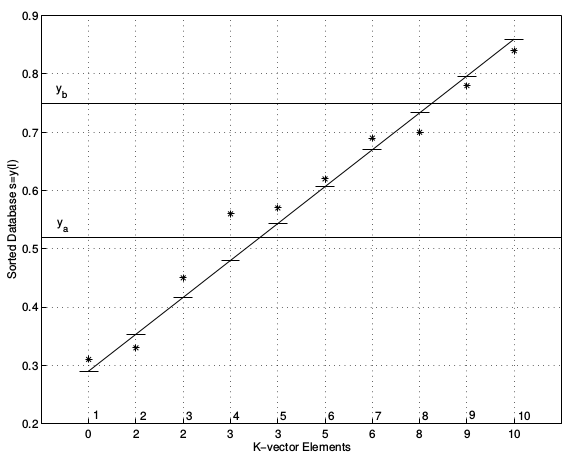
\includegraphics[scale=0.57]{k-vector-example.png}
\centering
\caption[K-vector technique example]{K-vector technique example, Image from \citep{mortari2000k}}
\label{fig:k-vector-example}
\end{figure}

In the Figure \ref{fig:k-vector-example} it is shown how such k-vector construction looks like. In this example the database has 10 elements. X-axis describes k-vector elements $\bm{k}(i)$ and y-axis describes the sorted values $\bm{s}(i)$ (inter-star angle in this case). The value of $\bm{k}(i)$ represents the number of elements of the database vector $\bm{y}$ below the value $z(i)$.
The resulting k-vector is $\bm{k} = \{0, 2, 2, 3, 3, 5, 6, 8, 9, 10\}^T$.

The following equations describe how the k-vector database is created. The line connecting two extreme points, $[1, y_{min}]$ and $[n, y_{max}]$, has to be a little stepper and connect points $[1, y_{min}-\delta\epsilon]$ and $[n, y_{max}+\delta\epsilon]$. This assures $\bm{k}(1) = 0$ and $\bm{k}(n	) = n$ and simplifies the code by avoiding many index checks.
\begin{equation}
z(x) = mx + q \begin{cases}m = \frac{y_{max} - y_{min} + \delta\epsilon}{n - 1} \\
q = y_{min} - m - \delta\epsilon \end{cases}
\end{equation}
\begin{equation}
\delta\epsilon = (n - 1)\epsilon
\end{equation}
$\epsilon$ is relative machine precision for double precision arithmetic
\begin{equation}
\epsilon \approx 22.2 \times 10^{-16}
\end{equation}
Each other element can be found using the following equation:
\begin{equation}
\bm{k}(i) = j \hspace{0.5cm} where \hspace{0.5cm} s(j) \leq z(i) < s(j + 1)
\end{equation}
or
\begin{equation}
\bm{k}(i) = j \hspace{0.5cm} \textnormal{where j is the greatest index such} \hspace{0.5cm} s(j) \leq \bm{y}	(\bm{I}(i)) \hspace{0.5cm} \textnormal{is satisfied.}
\end{equation}

At this point k-vector has been built, and further use is quite simple. The equation to find indices identifying in $\bm{s}$ vector all possible data within the range $[y_a, y_b ]$ is following:

\begin{equation}
j_b = \Big\lfloor\frac{y_a - q}{m}\Big\rfloor \hspace{0.5cm} and \hspace{0.5cm} j_t = \Big\lceil\frac{y_b - q}{m}\Big\rceil
\end{equation}
In the example of Figure \ref{fig:k-vector-example} it is $j_b = 4$ and $j_t = 9$. After indices are evaluated it is possible to calculate
\begin{equation}
k_{start} = \bm{k}(j_b) + 1 \hspace{0.5cm} and \hspace{0.5cm} k_{end} = \bm{k}(j_t)
\end{equation}

Finally, having found $k_{start}$ and $k_{end}$ it is immediately known, that searched elements are $\bm{y}(i) \in [y_a, y_b]$, which are all the $\bm{y}(\bm{I}(i))$ where $k$ ranges from $k_{start}$ and $k_{end}$.

Note that in example the searched elements should be $k_{start} = 4$ and $k_{end} = 8$ while the presented technique returns $k_{start} = 4$ and $k_{end} = 9$. This happens due to fact that $k_{start}$ and $k_{end}$ have $50\%$ possibility to not belong to the $[y_a, z(j_a +1)]$ and $[z(j_b), y_b)]$ ranges respectively.

\subsection{Attitude Determination}

The last main part of the star-tracker program is attitude determination. After star pattern is found, there are come two lists of unit vectors. One list is in the body frame while the other is in the inertial frame. In order to find rotation between them and later CubeSat's attitude, an attitude determination method must be applied. A number of techniques were designed to solve this problem. Typically the output can come in the form of a quaternion, Euler angles or a rotation matrix (\gls{dcm}).

The attitude determination methods should be fast and robust. This section describes few most common algorithms designed to solve this problem.


\subsubsection{TRIAD}

Three Axis Attitude Determination (TRIAD) is based on constructing two triads of orthonormal unit vectors using the vector information from input. Both triads are components of the same reference frame $F_t$ expressed in the body and inertial frames\cite{hall2003spacecraft}.

$\bm{w}_1$ and $\bm{w}_2$ are two vectors in body frame and $\bm{v}_1$ and $\bm{v}_2$ are in reference frame. First step of the algorithm is following:

\begin{subequations}
\begin{equation}
\bm{r}_1 = \bm{w}_1/|\bm{w}_1|
\end{equation}
\begin{equation}
\bm{r}_2 = (\bm{r}_1 x \bm{w}_2) /|\bm{r}_1 x \bm{w}_2|
\end{equation}
\begin{equation}
\bm{r}_3 = \bm{r}_1 x \bm{r}_2
\end{equation}
\end{subequations}

and the following matrices in reference frame:

\begin{subequations}
\begin{equation}
\bm{s}_1 = \bm{v}_1/|\bm{v}_1|
\end{equation}
\begin{equation}
\bm{s}_2 = (\bm{s}_1 x \bm{v}_2) /|\bm{s}_1 x \bm{v}_2|
\end{equation}
\begin{equation}
\bm{s}_3 = \bm{s}_1 x \bm{s}_2
\end{equation}
\end{subequations}

where $\bm{r}_i, i\in\{1, 2, 3\}$ are matrices in body frame and $\bm{s}_i, i\in\{1, 2, 3\}$ are matrices in reference frame.


Finally the attitude matrix $\bm{A}$ is computed:

\begin{equation}
\bm{A} = \bm{r}_1 \cdot \bm{s}_1^T + \bm{r}_2 \cdot \bm{s}_2^T + \bm{r}_3 \cdot \bm{s}_3^T 
\end{equation}


The disadvantage of this algorithm is discarding some of the information, therefore losing the accuracy. The main advantage is that TRIAD is quite fast.


\subsubsection{q-method}

In 1968 Paul Davenport applied Wahba’s problem to spacecraft attitude determination, via method called q-method\cite{keat1977analysis}. 

Let loss function be represented in quaternion form:

\begin{equation}
L(A) = \frac{1}{2} \sum |\bm{b}_i - D(\bm{q})\bm{r}_i|^2
\end{equation}

where quaternion $q$ is searched, that minimizes cost function $L$. Here, $q$ is the eigenvector corresponding to the largest eigenvalue of $K$ matrix, which is generated as follows:

\begin{subequations}
\begin{equation}
\sigma = \sum \bm{b}_i^T\bm{r}_i
\end{equation}
\begin{equation}
B = \sum \bm{b}_i\bm{r}_i^T
\end{equation}
\begin{equation}
S = B + B^T
\end{equation}
\begin{equation}
\bm{Z} = \sum \bm{b}_i x \bm{r}_i
\end{equation}
\end{subequations}

\begin{equation}
\bm{K} = \begin{bmatrix}
\bm{S} - \sigma\bm{I}_3 & \bm{Z} \\
\bm{Z}^T & \sigma
\end{bmatrix}
\end{equation}

$\bm{I}_3$ is 3x3 identity matrix.

\subsubsection{QUEST}

The quaternion estimation (QUEST) method was proposed by \citet{shuster1978approximate}. The method builds on the q-method. The main goal for this method was to develop the quaternion estimator was to obtain finding the optimal eigenvalue for the loss function. The eigenvalue problem is reformulated to problem of solving a characteristic equation. The minimization of loss function is following:

\begin{equation}
\begin{split}
J(\bm{q}) = \frac{1}{2}\sum_{j=1}^n\frac{1}{\sigma_j^2}(\bm{b}_j - \bm{R}_b^i(\bm{q})\bm{r}_j)^T(\bm{b}_j - \bm{R}_b^i(\bm{q})\bm{r}_j) = \\
\frac{1}{2}\sum_{j=1}^n\frac{1}{\sigma_j^2}(\bm{b}_j^T\bm{b}_j - 2\bm{b}_j^T\bm{R}_b^i(\bm{q})\bm{r}_j + \bm{r}_j^T\bm{r}_j)
\end{split}
\end{equation}

where $\bm{r}_j$ is unit vector given in the NED frame, while $\bm{b}_j$ is unit vector given in the fixed BODY frame. The parameter $\sigma_j$ is the standard deviation of the measurement error. Due to fact that both unit vectors have to be of equal length, the cost function can be reduced to:

\begin{equation}
J(\bm{q}) = \sum_{j=1}^n\frac{1}{\sigma_j^2}(1 - \bm{b}_j^T\bm{R}_b^i(\bm{q})\bm{r}_j)
\end{equation}

The main advantage is that QUEST method can find exact solution after one step. The method is designed to preserve quaternion normalization. The problem is that it is mostly estimation, hence some accuracy is not perfect.

\subsubsection{Singular Value Decomposition (SVD)}

This method was proposed by \citet{markley1988attitude}. It is not usually used while it output type is \gls{dcm}, not quaternions. It is used however for simulations, like for example by \citet{mcbryde2012star}.
Since the needed output from attitude determination must be quaternion, not \gls{dcm}, this method will not be used.
 
The algorithm works as follows:

Firstly the matrix $\bm{B}$ is calculated with $n$ observed stars, where $b_i$ is image star and $r_i$ catalogue star for real star $i$:
\begin{equation}
\bm{B = \sum_{i=1}^nb_ir_i^T}
\end{equation}
\gls{svd} of matrix $\bm{B}$ has to be found
\begin{equation}
\bm{B = USV^T}
\end{equation}
where matrices $\bm{U}$ and $\bm{V}$ are orthogonal and diagonal matrix of singular values $\bm{S}$.

Now the proper orthogonal matrices $\bm{U}_+$ and $\bm{V}_+$ using:
\begin{equation}
\bm{U}_+ = \bm{U}\begin{bmatrix}
1 & 0 & 0 \\
0 & 1 & 0 \\
0 & 0 & det\bm{U}
\end{bmatrix}
\end{equation}
\begin{equation}
\bm{V}_+ = \bm{V}\begin{bmatrix}
1 & 0 & 0 \\
0 & 1 & 0 \\
0 & 0 & det\bm{V}
\end{bmatrix}
\end{equation}
The \gls{dcm} $\bm{A}$ can be found by:
\begin{equation}
\bm{A = U_+V_+^T}
\end{equation}

\subsubsection{Other techniques}
There exist also other methods:
\begin{itemize}
\item The Fast Optimal Attitude Matrix\cite{markley1993attitude},
\item Predictive Attitude Determination\cite{crassidis1997predictive}.
\end{itemize}

However they are not very popular and not often used, therefore they will not be described here.

\subsubsection{Conclusions}


From all the presented methods, QUEST was selected due to low computational requirements and good accuracy in attitude estimation.

QUEST outperforms q-method in terms of speed\cite{markley1999estimate}, and while it is less accurate it still qualifies for satellite. Comparing to TRIAD, QUEST is more robust to noise. TRIAD is designed only for two vectors, hence in case of inaccurate measurements, it will yield erroneous result, even if there are more vector that could be used for estimation. According to \citet{ccelik2013comparison} the computational time and accuracy in q-method and TRIAD are comparable, hence QUEST is faster from both of them.

QUEST was also chosen by \citet{huffman2006designing} and \citet{tappe2009development} to be used on satellites' star-trackers.

\newpage
\section{Star-tracker program}

Star-tracker program was written in Python 3.6 under Anaconda distribution run on ARM processor (on Jetson TX2) with usage of numba library for easy GPU computation. The program has main file which is responsible for running whole program, and the rest is divided in three parts: star recognition - calculating centroids of stars from image and discarding the ones with too high magnitude; star identification - finding stars' catalog IDs and discarding false stars, using isolated Planar Triangle algorithm; attitude estimation using isolated QUEST algorithm. Additionally there is separate part for catalog generation for Planar Triangle algorithm.

During star-tracker development it was necessary to firstly create testing environment in order to ensure that program will work correctly. Each part of algorithm was tested separately on wide range of examples, then they were together as fully functioning star-tracker program.

During development k-vector algorithm was discarded because results of star identification with k-vector were inconsistent. Moreover for just 1500 stars it didn't give any visible speed advantage. It is possible it would be worth using in case of catalogs with more stars.

The Tracking Mode does not function properly and will have to be rewritten in the future version of star-tracker. Although correctly working Tracking Mode would make star-tracker faster, it is possible for it to work all the time in LIS mode.

Figure \ref{fig:star-tracker_diagram} shows general schema of designed star-tracker program.

\begin{figure}[!htbp]
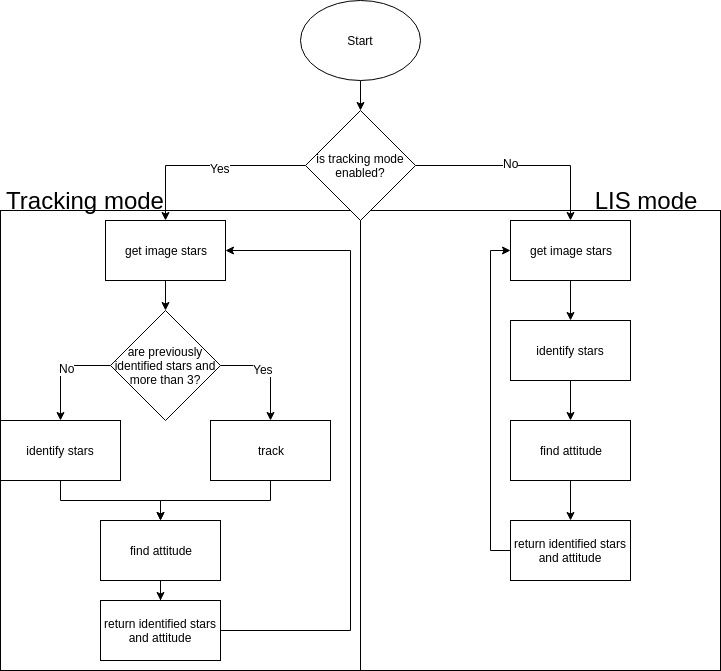
\includegraphics[scale=0.53]{startracker_full_diagram.jpg}
\centering
\caption{Designed star-tracker full program diagram}
\label{fig:star-tracker_diagram}
\end{figure}


\subsection{Program parts}

\subsubsection{Star Triangle Catalog}

The star triangle catalog was created with the following parameters:
- stars with max magnitude 5;
- FOV 10\degree
what gave 1625 stars which gave 44922 triangles.

In other work\cite{mortari2004pyramid} around 6000 stars were used to create catalog, hence another catalog was created with stars' magnitude 6.2, what gave 6279 stars and 1160853 triangles. This however proved to be both not accurate and a lot slower in testing than in case of smaller catalog, hence the smaller catalog was chosen to be used in this star-tracker program.

The small catalog is good enough, because it covers most of the sky with at least 3 stars. Tests prove that in random part of the sky with few magnitude 5 stars program is able to identify stars in around 90\% of cases. It is best if no star with magnitude greater than the given in the catalog would be passed from star centroid algorithm into star identifier, although star identifier can deal with some false stars with quite high accuracy.

The catalog has following columns:
\begin{enumerate}[noitemsep]
\item star 0 Hipparcos ID, 
\item star 1 Hipparcos ID,
\item star 2 Hipparcos ID,
\item area,
\item polar moment,
\item k-vector ID.
\end{enumerate}

\subsubsection{Star Catalog}

There was additional catalog created for stars only. It is used by Star Identifier for eliminating incorrect stars and by Orientation Finder as interial frame star vectors for LIS mode. The catalog was created with stars of max magnitude 6.2.

The catalog has following columns:
\begin{enumerate}[noitemsep]
\item star Hipparcos ID,
\item unit vector 1st element,
\item unit vector 2nd element, 
\item unit vector 3rd element.
\end{enumerate}

\subsubsection{Getting centroids of image stars}

First camera reads its input and gets image, which is later converted into matrix of light intensity values per pixel. After that program enters into centroiding algorithm. On GPU, each pixel is checked firstly for its light intensity value, average light intensity of neighboring pixels and if the pixel is not on the border. If all those conditions are passed, then pixel centroid is calculated for this pixel, according to the instructions in the previous chapter. After that pixel centroids are being clustered in order to merge neighboring centroids into one star centroid. Finally all found star centroids are converted to unit vectors.

Centroid algorithm was tested using images created with Stellarium, free planetarium software, which made possible to mock output from star-tracker camera. Images are with following parameters: FOV 10\degree and 900x900 pixels, and imitate parts of that should be visible by star-tracker on the actual orbit.

This is the most computation-consuming part of the program, however the usage of GPU made it quite fast.

On Jetson Centroiding lasts around 200 ms in most cases, but it can go up higher with more stars in the input image. It will also go much higher in images with higher resolution.

Computational complexity is $O(x*y*(\frac{mag_{pix}}{2}+\frac{a_{roi}}{2}))$, where:
\begin{itemize}[noitemsep]
\item $x$ is number of horizontal pixels,
\item $y$ is number of vertical pixels,
\item $mag_{pix}$ is amout of star magnitude pixels,
\item $a_{roi}$ is amout of ROI.
\end{itemize}

\begin{figure}[!htbp]
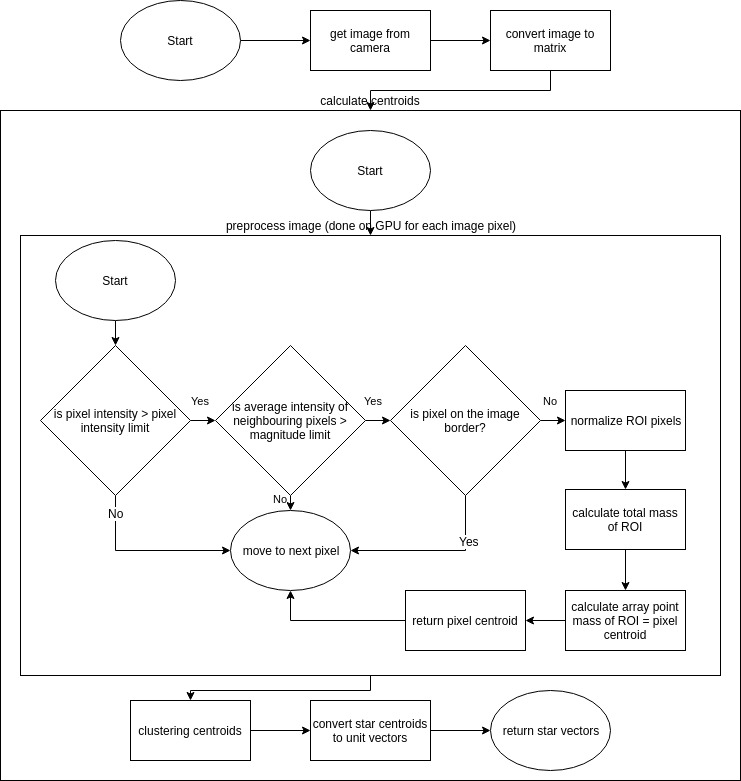
\includegraphics[scale=0.51]{get_image_stars_diagram.jpg}
\centering
\caption{Getting centroids of image stars diagram}
\label{fig:get_image_stars_diagram}
\end{figure}


\subsubsection{Star identification}
After having list of image star centroids in form of unit vectors program enters Star Identification phase. Firstly 3-star combinations are created, and for each combination all eligible stars are being found. It is done by calculating Planar Triangle for each 3-star combination and looking up all triangles in Star Triangle Catalog that are withing area and polar moment ranges. Each image star has a list of eligible stars, which is being extended after each lookup, i.e. each image star in the 3-star combination has added the same eligible stars to their lists. After doing this for all 3-star combinations, each image star has list with all eligible stars and one of the most common star IDs in the list should be Hipparcos star ID. Next step is done for each image star: take 10 most common eligible star IDs. If there are none, then this image star is identified as false star. If there are any eligible stars, then for each eligible star ID it is checked, whether this ID was already assigned to any other image star in this image. If it was not, then this eligible star ID is assigned to this image star as its Hipparcos star ID. If it was, then move to next most common eligible star ID. If this is the last most common eligible star, then this image star is identified as false star. After above steps are done for all image stars, the last step of stars identification takes place: removal of incorrect stars. For each image star with found Hipparcos star ID, those stars are looked up in Star Catalog together with their unit vectors. Next each pair of stars is checked if they actually even could be in the same image scene. This is done the same way as during Triangle Catalog creation, by checking if the dot product of unit vectors is higher or equal to the cosine of FOV. The stars which have been marked as incorrect most times are marked as false, the rest stays the same. After this step is finished, the program already has finished star identification and as result it returns list of image stars with information what is its Hipparcos star ID or if it is false star.

On Jetson Star Identification lasts up to 100-200 ms in most cases, but it can go much higher with more stars in the input image, even to 5 seconds. Possibly rewriting parts of this algorithm to use GPU would make it execute faster.

Computational complexity is $O(n^3+n^2)$, where $n$ is number of image stars.

Star Identifier algorithm was tested basing on ESA's star-tracker simulator created for competition needs\cite{esa-competition}. This simulator creates data two sets of data: one that would be the actual output of Centroiding algorithm, i.e. list of stars' centroids and magnitudes (x position, y position, magnitude); and the second set of data - list of stars' ids in Hipparcos catalog.
All tests were done with FOV 10\degree . On average algorithm using star triangle catalog of magnitude $\leqslant 5$ has accuracy above 90\%. Accuracy in this case means the percent of scenes in tests where no star was recognized incorrectly. It means that algorithm could also not recognize any star from the input data in given scene.
Such particular accuracy definition comes from the fact that for given scene no star can be recognized incorrectly in order to get correct result in the next part of program, which is QUEST algorithm. The percent of all identified stars in those test cases is around 95\% for stars within the catalog magnitude.

Test cases using star triangle catalog with magnitude $\leqslant 6$ proven to be also as accurate (\~95\%) for input data with stars with magnitude $\leqslant 5.56$, however the time of execution per scene rose significantly (from 50ms to 2.2s, 44 times). Test cases with input data with stars with magnitude $\leqslant 6$ has worsen the accuracy - less scenes without incorrectly identified stars comparing to the same test with catalog magnitude $\leqslant 5$, while time rose significantly (from 200ms to 4.9s, 24.5 times). In order to make this algorithm more accurate on higher magnitude stars it is necessary to explore options of rewriting parts of this algorithm to GPU, using k-vector and finding better constant values for Planar Triangle algorithm.


\begin{figure}[!htbp]
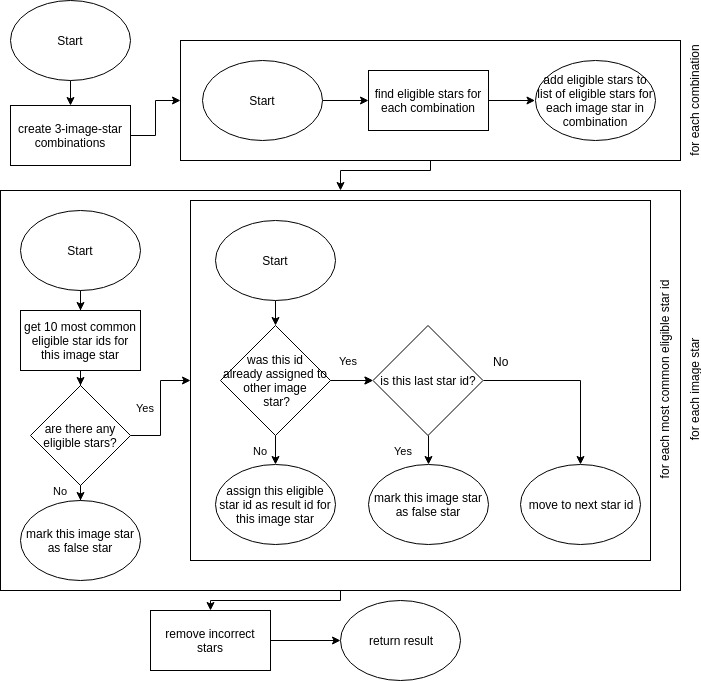
\includegraphics[scale=0.55]{star_identifier_diagram.jpg}
\centering
\caption{Star identification diagram}
\label{fig:star_identifier_diagram}
\end{figure}


\subsubsection{Finding attiude}
After having list of image stars with Hipparcos star IDs it is possible to determin attitude. For that there are two ways: in Tracking mode current star vectors are compared with previous star vectors; in LIS mode the current star vectors are compared with corresponding star vectors from Star Catalog. Attitude is calculated using QUEST algorithm. The QUEST algorithm was tested with example given in\cite{hall2003spacecraft} and gives identical result as in the book.

On Jetson Attitude Determination lasts below 10 ms in most cases, but it can go even up to 200 ms. This can happen if high percentage of stars in scene is misidentified and it takes more iterations to converge.

Computational complexity is $O(n)$, where $n$ is number of star vectors.

No block diagram will be presented for this part of the program, because it is just sequential calculating using equations in previous chapter.

\subsection{Example of working star-tracker}

This example is the first scene from "test full star-tracker" in the code. On the input Figure \ref{fig:example_0} is given - the image imitating what star-tracker should get from camera. Image was created using Stellarium program.

\begin{figure}[!htbp]
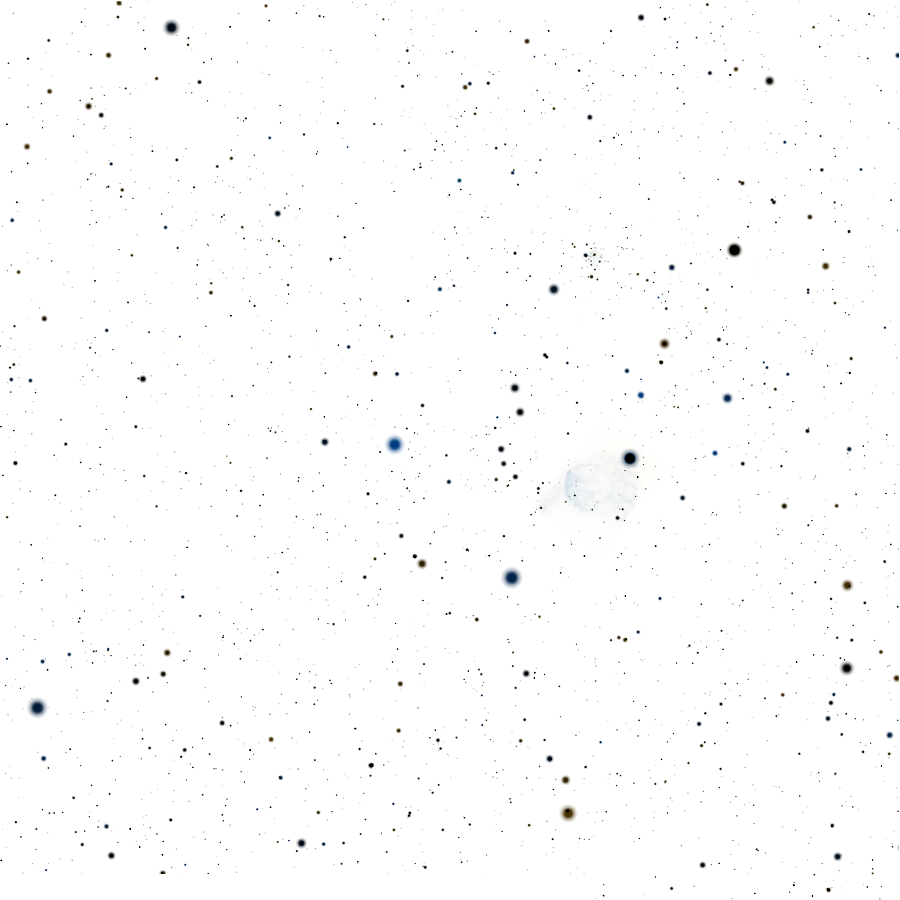
\includegraphics[scale=0.4]{example_0.png}
\centering
\caption[Example image input]{Example image input (colors were inverted for better visibility on paper)}
\label{fig:example_0}
\end{figure}

After recognizing stars in image and calculating their centroids, the data in Table \ref{fig:example_1} are obtained. Each star has assigned its image ID, vector values and image coordinates. 
The data are visualized in Figure \ref{fig:example_1}, where red numbers indicate image ID of stars in the image.


\renewcommand{\arraystretch}{1.5}
\begin{table}[!htbp]
\centering
\begin{tabular}{|c|c|c|c|c|c|}
\hline 
image ID & uv1 & uv2 & uv3 & pos x & pos y \\ 
\hline 
0 &  -0.0703 &  0.0227 & 0.997 &  567.0 &  86.9 \\
\hline 
1 &  -0.0423 &  0.0767 & 0.996 &  846.18 &  231.46 \\
\hline 
2 &   0.0009 & -0.0108 & 0.999 &  394.28 &  455.09 \\
\hline 
3 &  -0.0499 & -0.0799 & 0.995 &  37.00 &  191.95 \\
\hline 
4 &  -0.0248 &  0.0119 & 0.999 &  511.42 &  322.07 \\
\hline 
5 &   0.0817 & -0.0539 & 0.995 &  171.12 &  872.48 \\
\hline 
6 &  -0.0016 &  0.0348 & 0.999 &  629.57 &  441.50 \\
\hline 
7 &  0.0386 & 0.0550 & 0.997 & 734.03 & 649.48 \\
\hline 
\end{tabular}
\caption[Result of star recognition in the image]{Result of star recognition in the image - stars with unit vectors and image coordinates}
\label{tab:example_1}
\end{table}


\begin{figure}[!htbp]
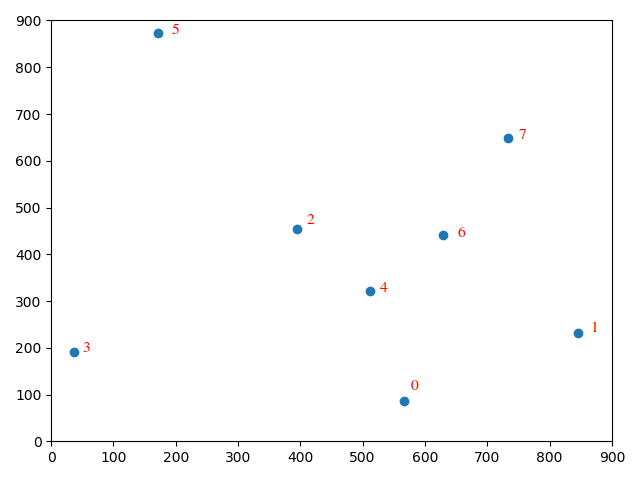
\includegraphics[scale=0.6]{example_1.png}
\centering
\caption[Result of star recognition]{Result of star recognition (red indicates image star ID assigned by algorithm)}
\label{fig:example_1}
\end{figure}

Next, for each combination of 3 image stars, eligible star are calculated and added list of eligible stars for each image star. Table \ref{tab:example_2} shows lists of eligible stars after doing it for all combinations. 
Only 10 most common occurrences of Hipparcos star ID are shown in the table due to long list. It is visible clearly, that stars 1 and 2 have significantly smaller number of highest occurring star ID.

\renewcommand{\arraystretch}{1.5}
\begin{table}[!htbp]
\centering
\begin{tabular}{|p{1.5cm}|p{1.5cm}|p{7cm}|}
\hline 
image ID & number of all stars & 10 most common stars (ID: amount), decreasing\\ 
\hline 
0 & 42 &  30883: 5, 29655: 3, 29696: 3, 30343: 2, 25737: 1, 26594: 1, 26727: 1, 34059: 1, 38500: 1, 38957: 1, ... \\
\hline 
1 & 24 &  26727: 2, 52468: 2, 56561: 2, 57363: 2, 25737: 1, 26594: 1, 86974: 1, 47391: 1, 87998: 1, 51849: 1, ... \\
\hline 
2 & 33 &  52468: 2, 34059: 1, 38500: 1, 38957: 1, 86974: 1, 47391: 1, 87998: 1, 51849: 1, 88267: 1, 47854: 1, ... \\
\hline 
3 & 75 &  32246: 7, 29655: 4, 52468: 3, 29696: 3, 30343: 3, 28734: 3, 57363: 2, 91919: 1, 92791: 1, 94713: 1, ... \\
\hline 
4 & 48 &  30343: 8, 29696: 4, 29655: 4, 32246: 3, 28734: 3, 30883: 2, 33856: 2, 91919: 1, 92791: 1, 94713: 1, ... \\
\hline 
5 & 57 &  29696: 9, 30343: 4, 29655: 4, 28734: 4, 30883: 3, 32246: 3, 34059: 1, 38500: 1, 38957: 1, 17304: 1, ... \\
\hline 
6 & 54 &  29655: 9, 32246: 4, 30343: 4, 29696: 4, 30883: 3, 28734: 3, 57363: 2, 57851: 2, 2912: 1, 4436: 1, ... \\
\hline 
7 & 63 &  28734: 7, 29696: 4, 30343: 3, 32246: 3, 29655: 3, 25737: 2, 57363: 2, 26594: 1, 26727: 1, 25302: 1, ... \\
\hline 
\end{tabular}
\caption{Eligible stars after combinations planar triangle}
\label{tab:example_2}
\end{table}

After that each image star is being assigned its Hipparcos ID according to algorithm described in previous chapter. 
The result is visible in Table \ref{tab:example_3}.

\renewcommand{\arraystretch}{1.5}
\begin{table}[!htbp]
\centering
\begin{tabular}{|c|c|c|c|c|c|c|}
\hline 
image ID & Hipparcos ID & uv1 & uv2 & uv3 & pos x & pos y \\ 
\hline 
0 &  30883 & -0.0703 &  0.0227 & 0.997 &  567.0 &  86.9 \\
\hline 
1 &  26727 & -0.0423 &  0.0767 & 0.996 &  846.18 &  231.46 \\
\hline 
2 &  52468 &  0.0009 & -0.0108 & 0.999 &  394.28 &  455.09 \\
\hline 
3 &  32246 & -0.0499 & -0.0799 & 0.995 &  37.00 &  191.95 \\
\hline 
4 &  30343 & -0.0248 &  0.0119 & 0.999 &  511.42 &  322.07 \\
\hline 
5 &  29696 &  0.0817 & -0.0539 & 0.995 &  171.12 &  872.48 \\
\hline 
6 &  29655 & -0.0016 &  0.0348 & 0.999 &  629.57 &  441.50 \\
\hline 
7 &  28734 & 0.0386 & 0.0550 & 0.997 & 734.03 & 649.48 \\
\hline 
\end{tabular}
\caption{Result of star identification before removing incorrect stars}
\label{tab:example_3}
\end{table}

To ensure the correctness of the data, the last part of star identification is executed: removing incorrect stars. 
Table \ref{tab:example_4} shows the most commonly appearing Hipparcos star IDs that could not be in the same image. 
Two IDs: 26727 and 52468 appear significantly more often than the rest of IDs, therefore they are going to be removed from the result and marked with ID "-1", because it represents false star. 
26727 and 52468 happen to be found Hipparcos star ID for image stars 1 and 2, respectively.

The image star 1 was not found, because it is star with Hipparcos ID 29650 and magnitude higher than limiting 5. Therefore program marked this star as false star. 
Similarly with image star 2 - it is Mars planet, not a star, hence program marked it also as false star.

The final result of star identification is visible in Table \ref{tab:example_5} and is visualized in Figure \ref{fig:example_5}. The red labels in the image are Hipparcos stars IDs and name of the planet Mars.

\renewcommand{\arraystretch}{1.5}
\begin{table}[!htbp]
\centering
\begin{tabular}{|p{7cm}|}
\hline 
26727: 7, 52468: 7, 28734: 2, 29655: 2, 29696: 2, 30343: 2, 30883: 2, 32246: 2 \\
\hline 
\end{tabular}
\caption{Hipparcos IDs of incorrect stars}
\label{tab:example_4}
\end{table}

\renewcommand{\arraystretch}{1.5}
\begin{table}[!htbp]
\centering
\begin{tabular}{|c|c|c|c|c|c|c|}
\hline 
image ID & Hipparcos ID & uv1 & uv2 & uv3 & pos x & pos y \\ 
\hline 
0 &  30883 & -0.0703 &  0.0227 & 0.997 &  567.0 &  86.9 \\
\hline 
1 & -1 & -0.0423 &  0.0767 & 0.996 &  846.18 &  231.46 \\
\hline 
2 & -1 &  0.0009 & -0.0108 & 0.999 &  394.28 &  455.09 \\
\hline 
3 &  32246 & -0.0499 & -0.0799 & 0.995 &  37.00 &  191.95 \\
\hline 
4 &  30343 & -0.0248 &  0.0119 & 0.999 &  511.42 &  322.07 \\
\hline 
5 &  29696 &  0.0817 & -0.0539 & 0.995 &  171.12 &  872.48 \\
\hline 
6 &  29655 & -0.0016 &  0.0348 & 0.999 &  629.57 &  441.50 \\
\hline 
7 &  28734 & 0.0386 & 0.0550 & 0.997 & 734.03 & 649.48 \\
\hline 
\end{tabular}
\caption{Final result of star identification}
\label{tab:example_5}
\end{table}


\begin{figure}[!htbp]
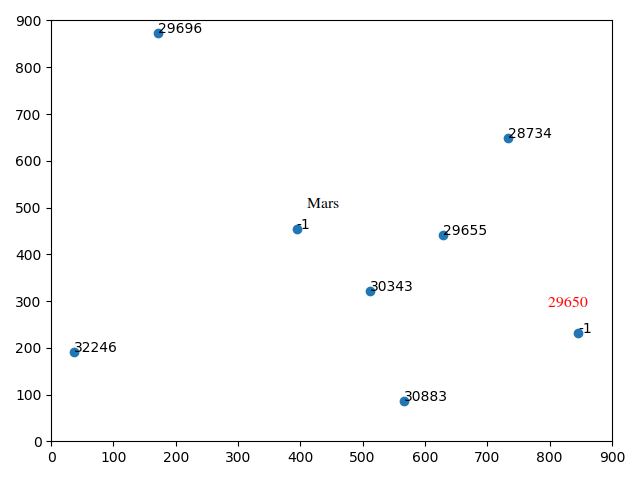
\includegraphics[scale=0.6]{example_2.png}
\centering
\caption[Final result of star identification]{Final result of star identification (black indicates the Hipparcos star ID found by algorithm, red indicates the real ID, "-1" indicates "false star")}
\label{fig:example_5}
\end{figure}


Finally the identified stars are used for calculating quaternion. The resulting quaternion is visible in Equation \ref{eq:example_6}, where the form of quaternion is described in Equation \ref{eq:code_quaternion}.

\begin{equation} \label{eq:example_6}
\bm{q} \coloneqq \begin{bmatrix}
-0.52101746 \\
-0.15332225 \\
-0.16303070 \\
 0.82368324
\end{bmatrix}
\end{equation}

The resulting quaternion can be translated to Euler angles as Right Ascension, Declination and Roll of the satellite in J2000 frame (Hipparcos catalog). The Equation \ref{eq:example_7} shows the result quaternion in Euler angles. Right Ascension is given in angle hours for easier applying in Stellarium program, where the result could be visualized. Figure \ref{fig:example_7} shows the attitude of satellite according to star-tracker, while Figure \ref{fig:example_8} shows the real attitude. The small difference could come from the imperfect transformation from quaternion to Euler angles.

\begin{equation} \label{eq:example_7}
\begin{split}
RA = 6h27m34.6927s \\
DEC = 24.990097882696112 \\
Roll = 63.100846657835916 \\
\end{split}
\end{equation}

\begin{figure}[!htbp]
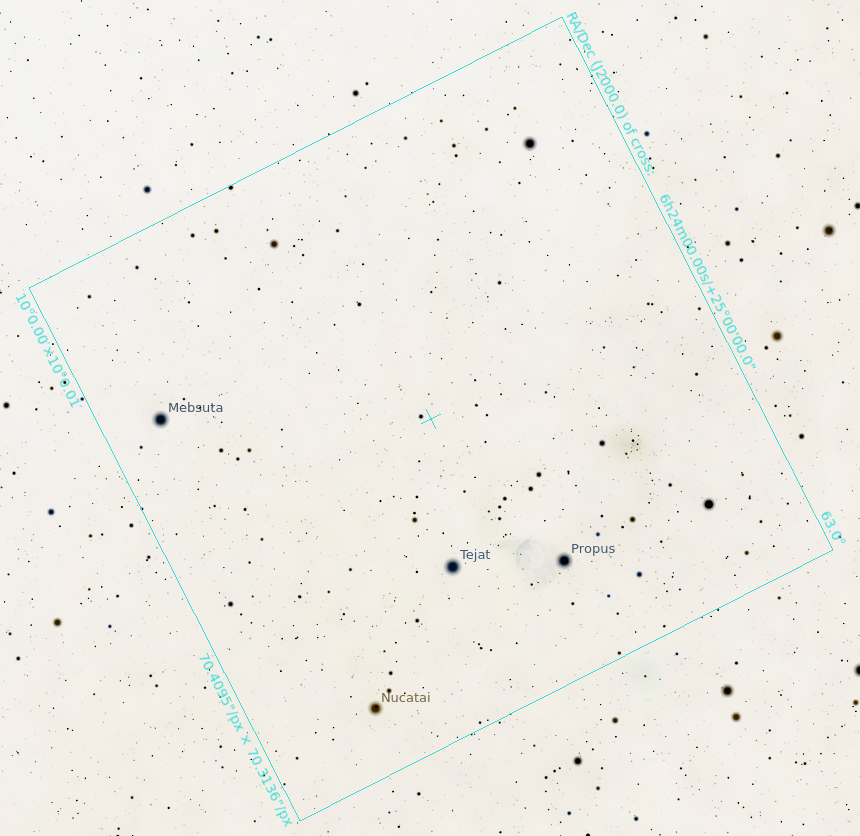
\includegraphics[scale=0.29]{example_3.png}
\centering
\caption[Attitude according to star-tracker]{Attitude according to star-tracker. The square frame is the FOV of star-tracker's camera}
\label{fig:example_7}
\end{figure}

\begin{figure}[!htbp]
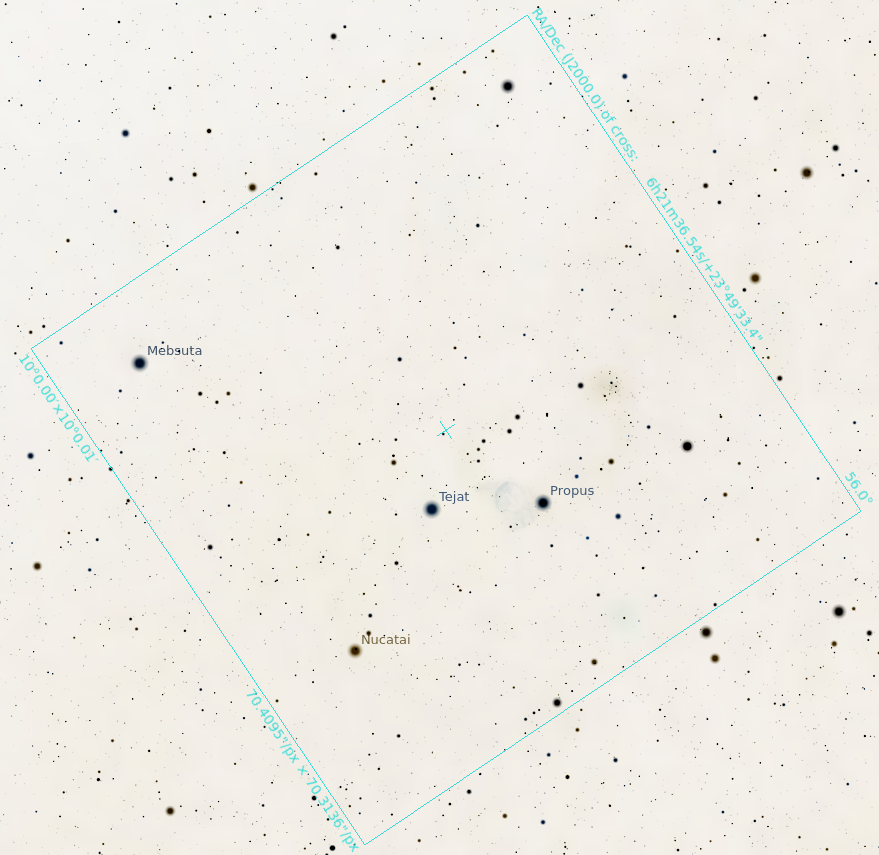
\includegraphics[scale=0.29]{example_4.png}
\centering
\caption[Real attitude]{Real attitude. The square frame is the FOV of star-tracker's camera}
\label{fig:example_8}
\end{figure}

\newpage
\section{Testing on NVIDIA Jetson TX2}

Testing of full star-tracker program was done in two ways:

First way of testing was to give image of sky on input and then to go through all parts of the program. The images were created using Stellarium program, which imitates part of sky with given FOV and coordinates. The parameters of images used during testing are FOV 10\degree , and resolution of 900x900 pixels.

Second way of testing was showing image of the sky on the separate screen and try to read it with camera on JETSON device. Although program clearly was able to find stars in the camera input, it needs precise configuration in order to find centroids accurately. Example of precise testing was done by \citet{tappe2011star}. Surely such testing will have to be done to test using this star-tracker program with dedicated camera.

The following results come from first way of testing: simulating input of star-tracker with already made images. The series of 14 images was run one by one. Figure \ref{fig:power_plot} shows the power consumption of algorithm on Jetson TX2. The values were collected by reading metrics collected by Ubuntu system while running the star-tracker test. The first peak is the loading of catalogs into the memory. At around 3rd second the first scene is read. Even with the highest load power consumption does not exceed 7 Watts. It is clearly visible that CPU consumption is significantly higher than GPU and is due to the fact that still most of star-tracker computation is done on CPU. High power consumption peaks in seconds 9-14 and 23-28 are due to the higher amount of stars in input scenes at that time, what leads to longer time of star identification process, which is the CPU consuming process.

Figure \ref{fig:times_plot} shows how much time was necessary to calculate attitude for each of 14 scenes. Scenes 2 and 12 have higher time of Attitude calculation because in those scenes quite big percentage of stars were misidentified and it took more iterations to finalize calculations. Enormously higher Star Identification times for scenes 10, 11 and 12 come from the much higher amount of stars in the scene image. 

Figure \ref{fig:power_times_plot} shows power consumption with marked times of each section calculation. Scene 10 takes time between 6th and 8th second and it is visible that power consumption raises a little. However in the next scene, scene 11 (seconds 8-13) the power consumption peaks from 5 to nearly 7 Watts. Scene 12 (seconds 13-18) also notes higher consumption, however smaller than previous scene. The next two scenes take very little time and around second 19 the next sequence of 14 images is started (red vertical line).

It is visible that the higher amout of stars on the input make program work significantly slower. While Cenotriding part needs rather the similar amount of time and Attitude Determination is not computationally expensive (takes longer only in case of misidentified stars, and still it was at most 200 ms), Star Identification can take even 40 times more than usual. The possible solution would be to rewrite Star Identification algorithm to be computed on GPU, especially because GPU power consumption stays on much lower level than CPU's.

NVIDIA Jetson TX2 seems to be good candidate to be used in space as the star-tracker hardware, however not for small CubeSats due to their low power budget. It could be used in little larger satellites, like in at least 6U CubeSats or HyperSats. Although existing star-trackers with dedicated hardware have much lower power consumption, even around 0.65-2.5 W, it is possible that optimization of star-tracker software would lower the power consumption. Jetson's low power consumption and GPU give possibility to create new star-tracker without spending time and resources on hardware part, but on software only. Possible Jetson could either be used to test machine learning solutions, or be used as the main on-board computer, what would lower the need for other devices on the satellite therefore lower the power consumption.

\begin{figure}[!htbp]
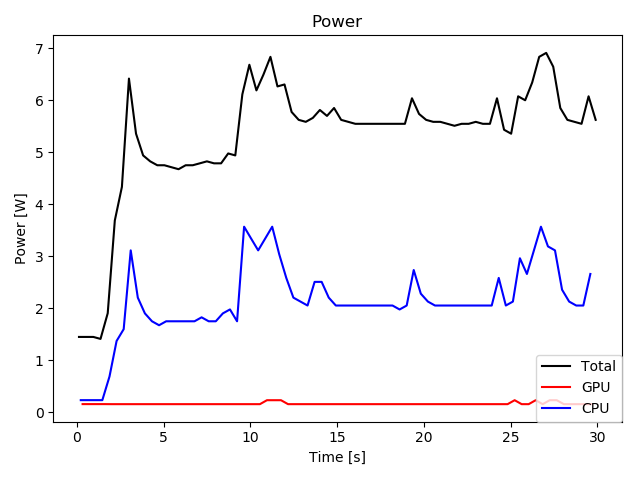
\includegraphics[scale=0.55]{power_plot.png}
\centering
\caption[Power consumption of star-tracker on Jetson TX2]{Power consumption of star-tracker on Jetson TX2}
\label{fig:power_plot}
\end{figure}

\begin{figure}[!htbp]
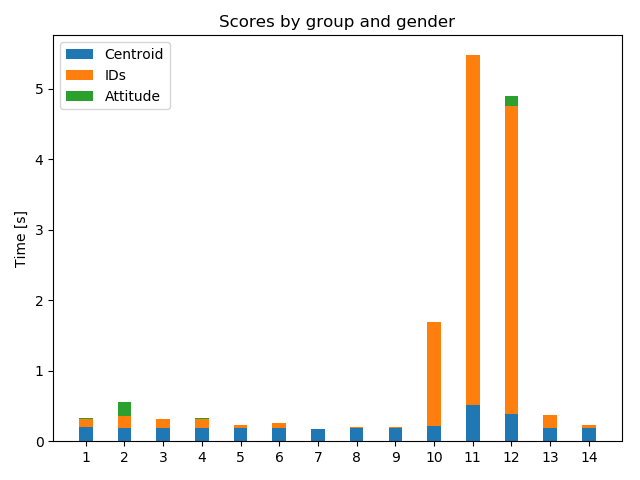
\includegraphics[scale=0.55]{times_plot.png}
\centering
\caption[Star-tracker execution time of each scene]{Star-tracker execution time of each scene}
\label{fig:times_plot}
\end{figure}

\begin{figure}[!htbp]
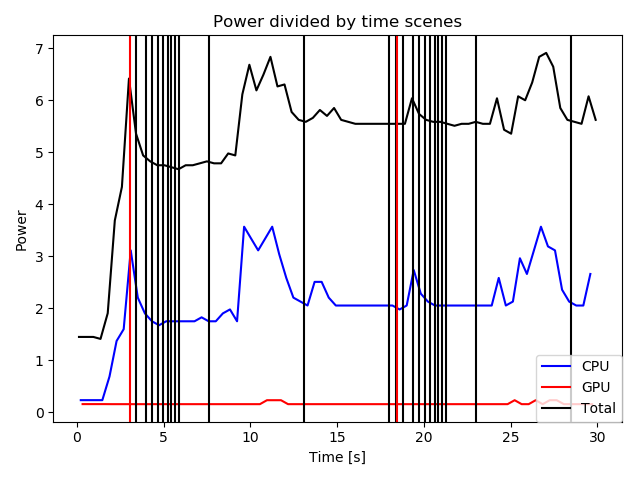
\includegraphics[scale=0.55]{power_times_plot.png}
\centering
\caption[Power consumption with marked scenes' computation times]{Power consumption with marked scenes' computation times. Red vertical lines mark start of next sequence of 14 input scenes, black vertical lines describe the start of next scene}
\label{fig:power_times_plot}
\end{figure}

\newpage
\section{Summary and future steps}

The program was tested using two sources of truth: images from Stellarium program and tests built basing on ESA's star-tracker simulator created for competition needs, what ensures high quality of tests. Testing indicated that all parts of star-tracker: star recognition in the images (centroiding), star identification with star catalog (planar triangle) and attitude determination (QUEST) work with high accuracy separately. The main goal of the thesis - star identification part - was thoroughly tested with few thousands mocked  scenes and few generated taken from Stellaris program. The speed of execution of the program shows that program could be used on the real satellite with refresh frequency at around $1Hz$ on average for LIS mode, and at least few times more with correctly working Tracking mode. The star-tracker is able to find attitude from the image of stars and calculate quaternion from it.

In order to use created star-tracker program on satellite the following things are necessary to be done:
\begin{itemize}
\item test with the dedicated camera,
\item run program in CPython implementation or rewrite program (or at least GPU parts) to C/C++ because the Python Anaconda distribution for ARM architecture is experimental and it could simply break on the satellite,
\item rerun catalog generation and test for the dedicated set of variables (FOV, etc.).
\end{itemize}

There exist a number of optional things to explore for bettering existing star-tracker:
\begin{itemize}
\item rewrite star identifier on GPU,
\item rewrite tracking mode to work more accurately,
\item optimize Planar Triangle algorithm,
\item catalog with more stars,
\item use k-vector algorithm for more stars,
\item explore other algorithms, especially for star identification and attitude estimation, because this is area which is being improved mostly.
\end{itemize}

NVIDIA Jetson TX2 seems to be good candidate to be used in space as the star-tracker hardware for slightly bigger satellites. With software optimization it could lower its consumption below 7 Watts, possibly even to around 5 Watts (power consumption under low CPU load). Other option is to use Jetson also instead of other devices what would lower the need for other components and would lower overall power consumption of satellite. Jetson can also be used for testing machine and deep learning solutions for star-trackers.
All goals set for this thesis have been met. Although there are few parts which could be improved, the existing star-tracker program works and could be with only few changes used on the real satellite. Additionally all the work done around the star-tracker program, like tests, etc., can be used for future development of even more accurate programs.


\newpage
\bibliographystyle{IEEEtranN}
\bibliography{IEEEabrv,bibfile}




\newpage

\listoftables

\newpage

\listoffigures

\newpage


\end{document}
